\documentclass[11pt]{article}
\usepackage[T1]{fontenc}
\usepackage{lmodern}
\usepackage[margin=1in]{geometry}
\usepackage{amsmath,amssymb,amsthm,mathtools}
\usepackage{microtype}
\usepackage[numbers,sort&compress]{natbib}
\usepackage{tikz}
\usetikzlibrary{arrows.meta,positioning,calc}
\usepackage[colorlinks=true,linkcolor=blue,citecolor=blue,urlcolor=blue]{hyperref}
\hypersetup{pdftitle={An Almost-Linear Approximation Scheme for Edit Distance},pdfauthor={OpenAI}}
\ifdefined\pdfinfoomitdate\pdfinfoomitdate=1\fi
\ifdefined\pdftrailerid\pdftrailerid{}\fi
\ifdefined\pdfsuppressptexinfo\pdfsuppressptexinfo=15\fi
\newtheorem{theorem}{Theorem}[section]
\newtheorem{lemma}[theorem]{Lemma}
\newtheorem{proposition}[theorem]{Proposition}
\newtheorem{corollary}[theorem]{Corollary}
\theoremstyle{definition}
\newtheorem{definition}[theorem]{Definition}
\theoremstyle{remark}
\newtheorem{remark}[theorem]{Remark}
\numberwithin{equation}{section}
\newcommand{\ED}{\operatorname{ED}}
\newcommand{\conn}{\operatorname{conn}}
\newcommand{\Lip}{\operatorname{Lip}}
\newcommand{\KL}{D_{\mathrm{KL}}}
\newcommand{\E}{\mathbb E}
\newcommand{\R}{\mathbb R}
\newcommand{\N}{\mathbb N}
\newcommand{\Z}{\mathbb Z}
\newcommand{\ind}{\boldsymbol 1}
\newcommand{\poly}{\operatorname{poly}}
\newcommand{\abs}[1]{\lvert#1\rvert}
\newcommand{\norm}[1]{\lVert#1\rVert}
\newcommand{\ceil}[1]{\lceil#1\rceil}
\newcommand{\floor}[1]{\lfloor#1\rfloor}
\newcommand{\pos}[1]{(#1)_+}

\title{An Almost-Linear Approximation Scheme for Edit Distance}
\author{OpenAI}
\date{September 24, 2026}
\begin{document}
\maketitle
\begin{abstract}
We give a uniform randomized approximation scheme for unit-cost edit distance.
For every fixed rational $\varepsilon\in(0,1)$, it estimates the distance
between arbitrary explicitly stored strings of total length $N$ within a
factor $1+\varepsilon$ with probability at least $2/3$, in worst-case expected
time $N^{1+o(1)}$ on a logarithmic-word RAM.
The algorithm supports polynomially bounded integer alphabets and returns zero
deterministically on equal strings.
\end{abstract}
{\small\tableofcontents}
\clearpage
\section{Introduction}\label{sec:intro}
The unit-cost edit distance $\ED(x,y)$ is the minimum number of
single-symbol insertions, deletions and substitutions that transform a string
$x$ into a string $y$. All three operations have cost one. The strings are
stored explicitly; write $N=|x|+|y|$. Their symbols are integer labels of
polynomial magnitude in $N+2$, stored in words of $O(\log(N+2))$ bits.
There is no bound on the alphabet size independent of $N$.

An approximation scheme receives a rational $\varepsilon\in(0,1)$ and
estimates the distance multiplicatively. Its guarantee must therefore include
returning zero when the two strings are equal. We prove the following result.

\begin{theorem}\label{thm:main}
There is one uniform randomized algorithm that, given $x,y$ and a rational
$\varepsilon\in(0,1)$, returns a nonnegative integer $\widehat D$ such that
\[
 \Pr\bigl[\ED(x,y)\le \widehat D\le(1+\varepsilon)\ED(x,y)\bigr]
 \ge \frac23.
\]
For every fixed rational $\varepsilon$, its worst-case expected running time
on strings of total length $N$ is $N^{1+o(1)}$ as $N\to\infty$ on the
logarithmic-word RAM. The expectation is over internal randomness only,
and the bound includes input processing, preprocessing, numerical work,
random sampling and all data-structure operations. Equal strings return zero
deterministically.
\end{theorem}

The program is uniform in the accuracy input. The asymptotic assertion is
pointwise in each fixed rational accuracy: its constants and the threshold
at which the bound applies may depend on $\varepsilon$. We do not assert
polynomial dependence on $1/\varepsilon$ or a joint bound when the accuracy
varies with $N$. The output is a distance estimate; no edit-script
reconstruction is needed.

The algorithm uses exact computation below an accuracy-dependent input-length
threshold. Section~\ref{sec:geometry} gives the finite input convention and
fallback rules; their thresholds are very large, so the result is an
asymptotic approximation scheme.

\subsection{Context and approach}
Edit distance originates in the study of errors in transmitted strings,
including Levenshtein's binary codes for insertions, deletions and bit
flips~\cite{Levenshtein1966}. The dynamic program of Wagner and
Fischer~\cite{WagnerFischer1974} computes the minimum cost of insertions,
deletions and substitutions in quadratic time. Masek and
Paterson~\cite{MasekPaterson1980} applied block tabulation to obtain a
logarithmic speedup for fixed alphabets and suitable fixed costs.
Distance-sensitive exact algorithms offer another route when few edits
are needed: Ukkonen~\cite{Ukkonen1985} developed bounded-distance methods,
and Landau and Vishkin~\cite{LandauVishkin1988,LandauVishkin1989} combined
furthest-reaching states with fast matching queries. Myers's related
difference algorithm~\cite{Myers1986} treats insertion--deletion scripts.
For unrestricted exact computation, Backurs and
Indyk~\cite{BackursIndyk2018} showed that a strongly subquadratic
deterministic algorithm
would refute the Strong Exponential Time Hypothesis. That lower bound
does not rule out fixed-factor approximation.

Approximation algorithms progressively improved the accuracy available
with substantially less work. In the following historical comparisons,
write $n$ for a common upper bound on the string lengths.
Batu and coauthors~\cite{BatuEtAl2003}
gave sublinear tests for fixed alphabets that distinguish sufficiently
small distance from linear distance. For general pairs, Bar-Yossef, Jayram, Krauthgamer and
Kumar~\cite{BarYossefEtAl2004} obtained an $n^{3/7}$ approximation in
quasi-linear time; Batu, Erg\"un and
Sahinalp~\cite{BatuErgunSahinalp2006} improved the factor to
$n^{1/3+o(1)}$. For binary strings, Ostrovsky and
Rabani~\cite{OstrovskyRabani2007}
constructed a low-distortion embedding into $\ell_1$, and Andoni and
Onak~\cite{AndoniOnak2012} obtained an efficiently computable
$2^{\widetilde O(\sqrt{\log n})}$ approximation in $n^{1+o(1)}$ time.
Andoni, Krauthgamer and Onak~\cite{AndoniKrauthgamerOnak2010} then
achieved a $(\log n)^{O(1/\xi)}$ factor in $n^{1+\xi}$ time for each
fixed $\xi>0$, using a hierarchical alignment representation and
nonuniformly allocated precisions.

The next advances reached constant factors. Chakraborty, Das,
Goldenberg, Kouck\'y and Saks~\cite{ChakrabortyEtAl2020} gave a
constant-factor approximation in $\widetilde O(n^{12/7})$ time.
Brakensiek and Rubinstein~\cite{BrakensiekRubinstein2020} and Kouck\'y
and Saks~\cite{KouckySaks2020} independently obtained near-linear
exponents for sufficiently far input pairs, with a material additive
error on general pairs. Andoni and Nosatzki~\cite{AndoniNosatzki2020}
removed that restriction: for every fixed $\xi>0$, their algorithm
gives an approximation factor depending only on $\xi$ in
$O(n^{1+\xi})$ time. The factor depends on the exponent parameter;
this is not an approximation scheme with error tending to zero.
For accuracy arbitrarily close to one, Mao and
Rubinstein~\cite[Theorem~6.1]{MaoRubinstein2026} recently obtained a
randomized $(1+\varepsilon)$ approximation in
$n^2/2^{\log^{\Omega(1)}n}$ time for every fixed positive
$\varepsilon$.

The issue addressed here is how to retain fixed $(1+\varepsilon)$
accuracy while reducing the expected total work to $N^{1+o(1)}$.
Recursive interval decompositions, economical evaluation of local
distances, and accounting along an optimal alignment have substantial
precedent in the algorithms above. In our refinement, unrestricted recursive evaluation of child distances would consume
the available time even if the resulting numerical error were small. We therefore need both a narrow family that
contains a suitable comparison alignment and a bound on the number of
child distances actually evaluated.

For the initial estimates we adapt the shift tree and precision sampling
of Andoni, Krauthgamer and
Onak~\cite{AndoniKrauthgamerOnak2010,AndoniKrauthgamerOnak2011}.
The refinement is related to Mao and Rubinstein's use of multiscale
deviation to constrain alignment paths before sampling
\cite{MaoRubinstein2026}. Here we measure the alignment's changes in relative position using
preliminary cost estimates as weights. A telescoping bound on their
variation controls the total cost of places where the prediction fails.
An entropy-regularized prediction rule, within the framework of
Rakhlin and Sridharan~\cite{RakhlinSridharan2013}, then controls the
accumulated error where the predictions can be used. We implement its
optimization by a finite Frank--Wolfe procedure
\cite{FrankWolfe1956,Jaggi2013}. The specialized geometric, probabilistic
and numerical guarantees are proved in this paper.

Two related comparisons concern different requirements on the output or
the edit costs. A single $\ell_1$ embedding of all binary strings up to a
length bound must incur growing distortion
\cite[Theorem~1.1]{OpenAIEditDistortion2026}. Our algorithm estimates the
distance of the supplied pair and does not construct such a common
embedding. Recent algorithms for metric-weighted edit costs obtain
$(3+\varepsilon)$ approximation in strongly subquadratic time
\cite{MaderTavasoliWang2026,DasKipouridisKociumaka2026}; their cost model
is broader than the unit-cost model treated here.

\subsection{Proof overview}
Recursively partition the first string into a tree of intervals, ending at
intervals of length at most one. An interval state consists of a source
interval $I$ and a target interval in the second string; its true cost is
the edit distance between the two substrings. An action at a nonleaf
assigns one target interval to each source child. We charge the sum of
the child estimates together with penalties for gaps or overlaps between
successive target endpoints and at the two outer endpoints. These
penalties let us compare nearby actions without requiring their target
intervals to join exactly.

\paragraph{Estimates that can be requested adaptively.}
The initial seed is an integer table whose entries give coarse upper
approximations to all interval-state costs. Although the algorithm evaluates
only requested entries, the accuracy event covers the entire domain:
later queries may depend on earlier random answers. Each initial entry
uses a private random stream, so its expected evaluation cost can also
be bounded conditional on the request that first exposes it. Accuracy
and expected work thus use different probability statements. Successive
refinement passes improve the seed approximation factor.

\paragraph{Predicting where an alignment goes.}
One refinement starts from such a seed. It first propagates estimates
through a wide family of actions and averages the resulting preliminary
tables to obtain cost proxies. At a source cut, the alignment's shift is
the target position minus the source position. The total shift change
divided by the predicted total cost suggests how this shift should evolve
as prefix cost accumulates. Requiring agreement with that prediction
restricts the possible target positions at each cut to a narrow band.
The algorithm computes these bands from the cost proxies alone.

To analyze them, fix optimal alignments and recursively round their child
endpoints. This gives a comparison tree that the algorithm never computes.
A cost-weighted variance measures how far the comparison shifts depart
from the predicted evolution. Its sum telescopes, with additional charges
for disagreements among the cost proxies. Consequently the total cost of
nodes with large discrepancies is controlled. At the other nodes, either
the substring-length difference already accounts for almost all predicted
cost, giving a direct error bound, or the computed band contains the
comparison action.

\paragraph{From a band to a better seed.}
Within a band, an entropy-regularized rule predicts an action using earlier
child values. Shared samples also compare rounded actions across nearby
representatives. The resulting estimates decrease with the refinement
index. After conditioning on complete child tables, the parent samples
retain their prescribed laws, and an online inequality bounds cumulative
excess over the comparison action.
Some intermediate estimates can be smaller than true cost. The analysis
therefore clips them from below at true cost, so an underestimate at one
node cannot cancel an error elsewhere. Summing
over the comparison tree gives a small expected positive error at any
fixed queried state, together with a deterministic multiplicative lower
bound. Independent repetitions, rescaling and medians turn these two
bounds into a simultaneous one-sided seed with a smaller approximation
factor. Repeating this improvement and making one final refinement gives
the desired answer.

\paragraph{Paying for recursive queries.}
A wide search or an optimization step may inspect many actions, but it
reuses previously gathered child values. Only shared group samples,
selected rounded actions and actual online draws require child values
at the current refinement index. Common rounded grids limit the number
of these calls to slightly more than the tree's branching factor.
Along a dependency path, a call either descends the tree at the same
index or decreases an index or pass. Counting these two kinds of steps
bounds the total expected work, including rational arithmetic and exact
sampling, by $N^{1+o(1)}$.

Section~\ref{sec:geometry} fixes the computational model, geometry and
parameters. Sections~\ref{sec:seed}--\ref{sec:bands} construct the tables.
Sections~\ref{sec:comparison} and~\ref{sec:regret} prove the geometric and
probabilistic estimates, and Section~\ref{sec:accuracy} assembles the
accuracy guarantee. Sections~\ref{sec:numerics} and~\ref{sec:work} implement
every operation and complete the running-time proof.

\section{Alignment geometry and computational parameters}\label{sec:geometry}
This section fixes the input conventions and the interval states used
throughout the algorithm. It also records the geometric inequalities that
allow child intervals to be combined even when their target endpoints do
not agree.

\subsection{Paths, states and connection costs}
Index string boundaries starting at zero. An alignment path has steps
$(1,0),(0,1),(1,1)$, of cost one, one, and the indicator that the two
characters on a diagonal step differ. Such a path gives an edit sequence.
Conversely, the original characters that survive an edit sequence occur in
the final string in their original order. Deleting other original
characters, inserting the remaining output characters and changing each
surviving character whose label differs gives an alignment of no greater
cost. Thus minimum alignment cost equals edit distance.

For an interval $I=(l,u]$ of the first string, an interval state is
$(I,q)$, where $q=(q^-,q^+)$ is an integer pair with
$0\le q^-\le q^+\le |y|$. When $I$ is fixed, we also call $q$ a state. Set
\[
 c(I,q)=\ED\bigl(x_{(l,u]},y_{(q^-,q^+]}\bigr),\qquad
 z(I,q)=(q^+-q^-)-(u-l).
\]
An endpoint's \emph{shift} is its target index minus its first-string index.
In particular, $z$ is the change in shift between the two endpoints.
For pairs use $|q-r|_1=|q^--r^-|+|q^+-r^+|$.

\begin{lemma}\label{lem:geometry}
For every interval state, $c(I,q)\ge |z(I,q)|$. Both $c(I,\cdot)$ and
$|z(I,\cdot)|$ are $1$-Lipschitz in the endpoint metric.
If $I$ is partitioned, in order, into $I_1,\ldots,I_m$, and
$\alpha=(s_1,\ldots,s_m)$ is any list of valid child states, define
\[
 \conn_r(\alpha)=|s_1^--r^-|
   +\sum_{i=1}^{m-1}|s_{i+1}^--s_i^+|+|s_m^+-r^+|.
\]
Then
\begin{align}
 c(I,r)&\le\sum_i c(I_i,s_i)+\conn_r(\alpha),\label{eq:connection}\\
 |z(I,r)|&\le\sum_i|z(I_i,s_i)|+\conn_r(\alpha).
 \label{eq:shift-connection}
\end{align}
The connection inequalities also hold for finite target intervals in any
extension of $y$ beyond its stored endpoints.
\end{lemma}
\begin{proof}
Only insertions and deletions change length, proving $c\ge|z|$.
Changing a target substring's endpoints costs at most $|q-r|_1$:
remove or insert endpoint portions if the substrings overlap, and delete
and insert the whole substrings if they are disjoint. The triangle
inequality gives the claim for $c$; the claim for $|z|$ follows from its
formula.

Edit each child to its specified target substring and concatenate the
results. Consider the walk on the target's boundary line that starts at
$r^-$, jumps to $s_1^-$, traverses each child target forward, makes the
successive connecting jumps, and ends at $r^+$. Expand each jump into unit
steps. From this walk choose, in order, one forward crossing of every unit
interval between $r^-$ and $r^+$. Successive first arrivals at the next
boundary give such a choice. The letters on these selected crossings,
in their walk order, form exactly the parent's target substring. Delete
the letters on unselected child crossings, and insert the letters on
selected connecting crossings. By net displacement, the number of
unselected forward crossings equals the number of backward crossings.
All backward crossings belong to connecting jumps, since child targets
are traversed forward. Thus deletions cost at most the total backward
jump length, while insertions cost at most the total forward jump length.
Their sum is $\conn_r(\alpha)$, proving~\eqref{eq:connection}.
This argument uses only the letters at finitely many target positions,
so it also proves the assertion for extensions of $y$.
Finally, sum the signed shift changes of child intervals and connecting
jumps and take absolute values to obtain~\eqref{eq:shift-connection}.
\end{proof}

Figure~\ref{fig:connection-cost} illustrates why the connection term permits
both gaps and overlaps between consecutive child targets.
\begin{figure}[htbp]
\centering
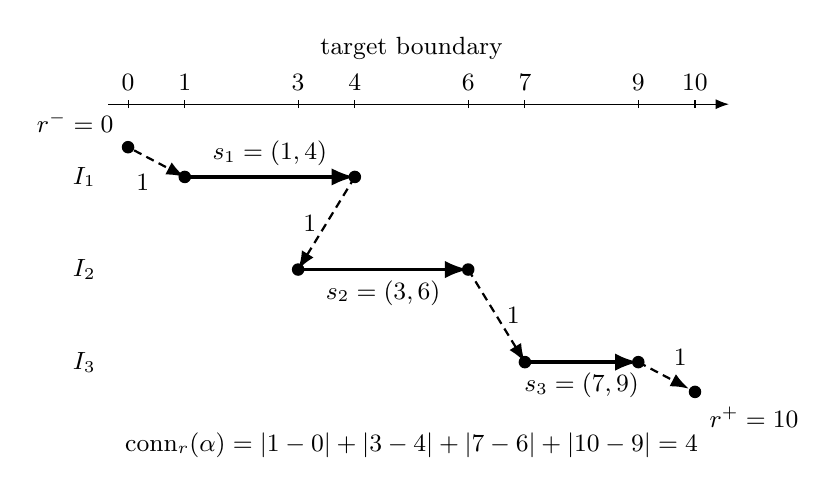
\begin{tikzpicture}[
  x=0.72cm,y=0.84cm,>=Latex,
  interval/.style={->,very thick},
  connection/.style={->,densely dashed,thick},
  endpoint/.style={circle,fill,inner sep=1.6pt},
  every node/.style={font=\small}]
\draw[->] (-0.35,1.1) -- (10.6,1.1);
\node at (5,1.95) {target boundary};
\foreach \t in {0,1,3,4,6,7,9,10} {
  \draw (\t,1.04) -- (\t,1.16);
  \node[above] at (\t,1.16) {$\t$};
}
\node[left] at (-0.4,0) {$I_1$};
\node[left] at (-0.4,-1.4) {$I_2$};
\node[left] at (-0.4,-2.8) {$I_3$};
\draw[interval] (1,0) -- (4,0)
  node[midway,above] {$s_1=(1,4)$};
\draw[interval] (3,-1.4) -- (6,-1.4)
  node[midway,below] {$s_2=(3,6)$};
\draw[interval] (7,-2.8) -- (9,-2.8)
  node[midway,below] {$s_3=(7,9)$};
\foreach \x/\y in {1/0,4/0,3/-1.4,6/-1.4,7/-2.8,9/-2.8}
  \node[endpoint] at (\x,\y) {};
\node[endpoint,label=above left:{$r^-=0$}] (start) at (0,0.45) {};
\node[endpoint,label=below right:{$r^+=10$}] (finish) at (10,-3.25) {};
\draw[connection] (start) -- (1,0) node[midway,below left] {$1$};
\draw[connection] (4,0) -- (3,-1.4) node[midway,left] {$1$};
\draw[connection] (6,-1.4) -- (7,-2.8) node[midway,right] {$1$};
\draw[connection] (9,-2.8) -- (finish) node[midway,above right] {$1$};
\node[align=center] at (5,-4.05)
  {$\conn_r(\alpha)=|1-0|+|3-4|+|7-6|+|10-9|=4$};
\end{tikzpicture}
\caption{Connection charges for three consecutive source children.
Solid arrows show their prescribed target intervals; dashed arrows join
these intervals in child order, with the outside endpoints $r=(0,10)$.
The jump from $4$ to $3$ points backward, so this walk is not itself an
alignment path. Lemma~\ref{lem:geometry} gives
$c(I,r)\le\sum_{i=1}^3c(I_i,s_i)+4$.
Only the horizontal target-coordinate displacement of a dashed arrow is
charged; the vertical separation of rows is for display.}
\label{fig:connection-cost}
\end{figure}


\subsection{Uniform access to the accuracy input}
The rational accuracy is supplied in a fixed canonical binary encoding of
its positive numerator and denominator in lowest terms, on a separate
read-only input.
For example, encode a positive integer by its binary length in unary,
a delimiter, and its binary digits, and concatenate the two encodings.
The input is promised to specify $0<\varepsilon<1$. Prefix inspection is
ordinary input access; no numerical operation on the rational is free.

The algorithm first handles equality, empty strings and $|x|\le1$
exactly. These cases require $O(N+1)$ string work. On other inputs define
$H$ as the least power of two at least $\lceil\log_2(N+2)\rceil$, and
$\ell$ as the least power of two at least $\max(1,\log_2 H)$.
Inspect at most $H^2+O(1)$ bits of the accuracy input. If its complete
encoding has not been obtained, use exact alignment dynamic programming.
The unread suffix is neither copied nor addressed. All addresses actually
used for this prefix have $O(\log(N+2))$ bits. If the encoding is obtained,
its integers have $O(H^2)$ bits, and exact arithmetic decides the test
$\ell\varepsilon\ge10$ with polynomial work in $H$.

Use exact dynamic programming also if $\ell<2^{1000}$ or
$\ell\varepsilon<10$. It uses $O((N+1)^2)$ word operations and can store
only two rows. Together with the bounded parameter inspection, this
charges every operation in these branches. For each fixed rational
encoding, the inspection bound eventually exceeds its length, and both
numeric tests eventually pass as $N$ grows. Thus the exact branches affect
only a bounded range of $N$ for each fixed $\varepsilon$. They preserve
the uniform algorithm and its approximation guarantee on that range.
No assertion about efficient joint dependence on encoding length or
$1/\varepsilon$ is needed.

\subsection{Parameters and the fixed interval tree}
All remaining arguments concern the large-input branch. Logarithms with
subscript two are binary, and $\ln$ denotes the natural logarithm.
The coarse estimator and interval tree use the branching factors $B$ and
$M$ below. The factor $A_{\rm init}$ is the initial seed accuracy, $F$
controls its reduction across passes, and $P$ controls endpoint-grid
resolution:
\begin{align*}
 p_*&=\left\lfloor(\log_2\ell)^{1/4}\right\rfloor,
 &B&=H^{p_*},&A_{\rm init}&=H^{p_*+4},\\
 M&=2^{\lfloor(\log_2 H)/20\rfloor},
 &P&=H^{p_*+20},&F&=\ell.
\end{align*}
The counts $T$ and $S$ govern preliminary propagation and refinement
iterations, respectively. The slopes $L_0$ and $L$ penalize changes in
target endpoints:
\[
 T=2^{\lceil(3/4)\log_2H\rceil},\qquad S=H/\ell^2,
 \qquad L_0=32F,\qquad L=128F.
\]
Finally, fix the error tolerances and the sampling and optimization
parameters. Their roles are specified at the corresponding constructions:
\begin{align*}
 \delta&=\ell^{-10},&\kappa&=\tau=\ell^{-4},
 &\theta&=\ell^{-40},\\
 \gamma&=\ell^{-20},&\eta&=\ell^5,&Q_1&=\ell^{80}.
\end{align*}
The essential separation is between $H=\Theta(\log(N+2))$ and
$\ell=\Theta(\log H)$: the branching factors and grid resolutions are
powers of $H$, while the tolerances are powers of $\ell$. The inequalities
below quantify the slack available between these scales.

Every integer parameter here is computable using bit lengths and integer
tests. For example, $p_*$ is the largest integer whose fourth power is
at most the integer $\log_2\ell$. The displayed fractional powers and
logarithms require no real-arithmetic oracle. All parameters used as dyadic
grid spacings are powers of two, and $S$ is a positive integer in this
branch.

We will repeatedly use the generous bounds
\begin{equation}\label{eq:parameter-slack}
 H\ge2^{\ell/2},\qquad \ell^{200}\le H^{1/100},\qquad
 p_*+21\le\sqrt\ell.
\end{equation}
The first follows from the definition of $\ell$; the other two follow at
$\ell\ge2^{1000}$ and become stronger as $\ell$ increases. More explicitly,
$200\log_2\ell\le\ell/200$ and
$(\log_2\ell)^{1/4}+21\le\sqrt\ell$ hold at this cutoff, and their
right sides thereafter grow faster. Factors polynomial in $\ell$ and
$p_*$ will consequently be much smaller than any fixed positive power
of $H$ needed below.

Partition $x$ into a complete $M$-ary tree of height
\[
 J=\left\lceil\log_M\max(1,|x|)\right\rceil.
\]
At a node $(l,u]$ use cuts
$l_i=l+\lfloor i(u-l)/M\rfloor$, $0\le i\le M$.
Empty intervals are allowed, and node labels distinguish repeated
intervals. Nodes need only be generated when requested. At depth $j$ the
width is at most $\lceil|x|/M^j\rceil$, and leaves have width at most one.
The parameters give
\begin{equation}\label{eq:tree-bounds}
 J\le100H/\ell,\qquad M^J\le M\max(1,|x|).
\end{equation}
Indeed $\log_2M\ge (\log_2H)/20-1$ and
$\log_2H\ge\ell/2$, whereas $\log_2|x|\le H$.
The second bound follows directly from the ceiling defining $J$.

At a leaf of width zero the exact cost is the target length. At a leaf
containing one character, the cost is one for an empty target, and otherwise
is the target length minus the indicator that this character occurs there.
Sort the pairs (symbol, position) of $y$ lexicographically by comparison
sorting. A binary search then tests occurrence in any target interval in
$O(\log(N+2))$ time, with $O(N\log(N+2))$ preprocessing work and linear
storage. The word-label assumption makes each comparison a bounded number
of word operations. Fresh padding symbols used later can be represented by
a tag together with a label; no search for an unused alphabet value is
needed.

All subsequent tables are indexed by this fixed tree and valid endpoint
pairs. The total domain is polynomial in $N+2$: there are at most
$2M^J$ nodes and at most $(|y|+1)^2$ pairs per node. A simultaneous
probability guarantee over this domain is meaningful even though the
algorithm will evaluate only a small part of it.

\section{Simultaneous coarse estimates}\label{sec:seed}

The refinement will need an integer estimate at every interval state, including
states chosen adaptively by later computations.  We construct these estimates
as a random table, while evaluating only the entries that are requested.  The
construction builds on tree and precision-sampling ideas of Andoni,
Krauthgamer, and Onak~\cite{AndoniKrauthgamerOnak2010}; the complete bounds
needed here are proved below.

\begin{theorem}[Initial estimates]\label{thm:seed}
With the parameters and labeled interval tree of Section~\ref{sec:geometry},
there is a lazily evaluated random table $U^{(0)}(I,q)$ of integers in $[0,N]$
such that, with probability at least $0.99$, simultaneously at every state,
\begin{equation}\label{eq:seed-guarantee}
 c(I,q)\le U^{(0)}(I,q)\le A_{\mathrm{init}}c(I,q).
\end{equation}
Every zero-cost state has value zero on every execution.  Conditional on any
first request for an entry and the previously exposed randomness, its expected
evaluation cost is at most $(1+|I|)2^{o(H)}$, uniformly in the state.  This cost
bound includes arithmetic and random sampling and does not require
\eqref{eq:seed-guarantee} to hold.
\end{theorem}

\subsection{A deterministic shift tree}

The hierarchical representation below is an adaptation of the
E-distance of Andoni, Krauthgamer and Onak~\cite[Definition~3.2 and
Theorem~3.3]{AndoniKrauthgamerOnak2010}. We prove its precise bounds here,
including the treatment of unequal lengths, empty intervals and bounded
integer shifts.

Fix one state and write $n_x=|I|$, $n_y=q^+-q^-$, and $c=c(I,q)$.  If
$n_y>2n_x$, return $n_y$: the bounds $n_y-n_x\le c\le n_y$ give the required
factor two.  Otherwise
test equality directly and return zero when the strings agree.  These steps
cost $O(1+n_x)$, since in the branch requiring character comparisons
$n_y\le2n_x$.  They include the case $n_x=0$.

For the remaining case, pad the shorter string at its right end with a fresh
tagged symbol to obtain two strings of the same length $n\le2n_x$.  Denote their
distance by $d$.  The length gap is at most $c$, so $d\le2c$.  Conversely,
remove padding from any padded alignment.  A diagonal joining padding to a
real character has cost one and can be replaced by an insertion or deletion
of the same cost; other operations consuming padding can be removed.  Hence
\begin{equation}\label{eq:padding-comparison}
 1\le c\le d\le2c,\qquad 1\le n\le N,\qquad d\le n.
\end{equation}
The last bound follows by substituting characters position by position.

For each dyadic guess
\[
 k\in\{1,2,4,\ldots,2^{\ceil{\log_2 n}}\},
\]
split the first padded string in a complete balanced $B$-ary tree of depth
$D_0=\ceil{\log_B n}$.  Its leaves have width zero or one.  Allowed shifts are
the integers in $[-k,k]$.  At a width-one leaf $w$ starting at position $j$,
let $T_w(v)$ be the mismatch indicator between its character and position
$j+1+v$ of the second padded string.  A position outside the latter string
has a virtual symbol that always mismatches.  At a width-zero leaf put
$T_w(v)=0$.  At an internal node define
\begin{equation}\label{eq:coarse-tree}
 T_w(v)=\sum_{i=1}^B\min_{v'\in[-k,k]\cap\Z}
       \{T_{w_i}(v')+2|v-v'|\}.
\end{equation}
Constant shifts show that $0\le T_w(v)\le |w|$, where $|w|$ denotes the node's
width.

The virtual symbols are chosen outside the alphabets of both padded
strings. Thus every leaf value is an edit cost against a finite interval
of an extended target string, to which Lemma~\ref{lem:geometry} applies.

\begin{lemma}\label{lem:shift-tree}
At the root $o$,
\[
 d\le T_o(0),\qquad
 T_o(0)\le(1+2BD_0)d\quad\hbox{if }k\ge d.
\]
\end{lemma}
\begin{proof}
The recurrence minimizes the sum of leaf mismatches and twice the total
absolute shift difference along tree edges, with root shift zero.  For any
assignment, concatenate the shifted leaf target intervals.  By traversing
the tree in depth-first order, the sum of jumps between consecutive leaf
intervals, including the connections to the outer endpoints, is at most
twice the sum of edge shift differences.  The connection inequality from
Section~\ref{sec:geometry}, including its virtual-position version, therefore
bounds $d$ by the assignment's cost.  This proves the first assertion.

For the second, fix an optimal padded alignment and choose ordered points
$(j,b_j)$ at every source cut, with $b_0=0$ and $b_n=n$.  Assign shift $b_j-j$
to every node starting at $j$.  Its absolute value is at most $d$, because
only insertion and deletion steps change the shift.  These assignments are
allowed when $k\ge d$.

For each child, the shift difference from its parent is at most the cost of
the alignment subpath between their chosen starting points, and thus at most
the cost of the parent's subpath.  There are $B$ children per parent; the
parent subpaths at each depth partition the alignment.  Edge differences
therefore sum to at most $Bd$ at each of the $D_0$ depths.  A mismatching
width-one leaf has positive cost in its corresponding subpath: a zero-cost
subpath would be a matching diagonal.  Leaf mismatches sum to at most $d$,
and width-zero leaves contribute nothing.  The assignment has total cost at
most $(1+2BD_0)d$.
\end{proof}

\subsection{Pruning and precision sampling}

Nonuniform additive precision is the sampling principle developed by
Andoni, Krauthgamer and Onak~\cite[Lemma~3.12]{AndoniKrauthgamerOnak2010}
and refined in~\cite[Lemma~1.2]{AndoniKrauthgamerOnak2011}, with earlier
multiscale sampling antecedents in Indyk and
Woodruff~\cite{IndykWoodruff2005}. The reconstruction arguments of Andoni,
Krauthgamer and Onak already allow estimates to depend on the sampled
precisions. Here we use a finite threshold
distribution and prove an event covering all potential interval states,
together with the conditional cost of a first request.

Computing all of \eqref{eq:coarse-tree} would be too expensive. The guess
$k$ will also serve as an additive allowance at the root: on one event
of high probability, we will obtain an estimate $\widetilde T_o$ between $T_o/2-k$ and
$2T_o+k$ simultaneously for every entry and guess. Then
$2(\widetilde T_o(0)+k)$ is an upper bound on $d$ for every guess,
and the guess $d\le k<2d$ gives an $O(1+BD_0)$ approximation.
We can therefore replace a node by zero whenever its entire cost fits
within its additive allowance. Larger guesses permit more pruning;
their larger allowances are paid back in the returned estimate. Set
\[
 Q_0=H^4,\qquad \lambda=\frac1{64H},\qquad a_o=k.
\]
At a node with allowance $a_w$, independently for its children draw
$R_i$ uniformly from $\{1,\ldots,B\}$ and set
\begin{equation}\label{eq:coarse-threshold}
 t_i=\frac{a_wR_i}{BQ_0},\qquad a_{w_i}=\lambda t_i.
\end{equation}
All these random choices can be defined in advance, even below nodes that
will be pruned.  The implementation exposes only those it needs.

If $|w|\le a_w$, use the identically zero estimate $\widetilde T_w$.  At any
other leaf use its exact array.  At an unpruned internal node first compute
\[
 \widehat s_i(v)=\min_{v'\in[-k,k]\cap\Z}
       \{\widetilde T_{w_i}(v')+2|v-v'|\},
\]
and then put
\begin{equation}\label{eq:coarse-estimate}
 \widetilde T_w(v)=\sum_{i=1}^B
     \ind_{\widehat s_i(v)\ge t_i}
     \max\{\widehat s_i(v),a_w/Q_0\}.
\end{equation}
The descendants used to compute $\widehat s_i(v)$ depend on $t_i$, so
these child estimates cannot be treated as fixed in a concentration
bound. The proof below first compares their sampled contributions with
two lists formed from true child costs. It then concentrates those lists
without assuming that any child estimate is accurate.

\begin{lemma}\label{lem:coarse-precision}
Except on an event of probability less than $0.01$, simultaneously for all
initial entries, all guesses, all their nodes, and all shifts,
\begin{equation}\label{eq:coarse-accuracy}
 T_w(v)/f_w-a_w\le\widetilde T_w(v)\le f_wT_w(v)+a_w,
 \qquad
 f_w=\left(\frac{1+\lambda}{1-\lambda}\right)^{\operatorname{height}(w)}
 \le2.
\end{equation}
\end{lemma}
\begin{proof}
Fix an internal node and a shift, and write $s_i$ for the true child penalty minimum
in \eqref{eq:coarse-tree}. Let $f'$ be the factor in
\eqref{eq:coarse-accuracy} at its children's structural height. Both $s_i$
and $f'$ are independent of all thresholds. Suppose for the moment that
the child accuracy inequalities hold with this factor. Adding a nonnegative
penalty preserves the lower bound after division by $f'$ and the upper
bound after multiplication by $f'$.  Taking minima gives
\[
 s_i/f'-\lambda t_i\le\widehat s_i(v)\le f's_i+\lambda t_i.
\]
Let $u=a_w/Q_0$ and define
\[
 \phi_i(h)=\ind_{h\ge t_i}\max\{h,u\},\qquad
 h_i^- =\frac{s_i}{f'(1+\lambda)},\qquad
 h_i^+=\frac{f's_i}{1-\lambda}.
\]
If $h_i^-\ge t_i$, then
$\widehat s_i(v)\ge(1+\lambda)h_i^--\lambda t_i\ge h_i^-$.
If $\widehat s_i(v)\ge t_i$, then
$\widehat s_i(v)\le f's_i+\lambda\widehat s_i(v)$, and consequently
$\widehat s_i(v)\le h_i^+$.  These implications prove the pathwise sandwich
\begin{equation}\label{eq:threshold-sandwich}
 \phi_i(h_i^-)\le\phi_i(\widehat s_i(v))\le\phi_i(h_i^+).
\end{equation}

We now establish concentration independently of the supposition about child
accuracy.  Conditional only on ancestor thresholds, $u$ is fixed and
$t_i=uR_i/B$ are independent.  For either of the two fixed argument lists
$h_i=h_i^\pm$, if $0\le h_i<u$ then
\[
 \phi_i(h_i)=u\,\operatorname{Bernoulli}
       \left(\frac{\floor{Bh_i/u}}B\right);
\]
if $h_i\ge u$, it equals $h_i$ deterministically.  Thus
\[
 0\le h_i-\E\phi_i(h_i)\le u/B,\qquad
 \operatorname{Var}(\phi_i(h_i))\le uh_i,
 \qquad |\phi_i(h_i)-\E\phi_i(h_i)|\le u.
\]
Write $V=\sum_i h_i$ and $Z=\sum_i\phi_i(h_i)$.  The total bias is at most
$u$.  Bernstein's inequality~\cite[Theorem~4.16]{Tropp2021Probability} at
deviation $z=\lambda V+a_w/2$ gives
\[
 \Pr(|Z-\E Z|>z)
 \le2\exp\left(-\frac{z^2}{2uV+(2/3)uz}\right)
 \le2\exp(-\lambda Q_0/12).
\]
For the last inequality, if $V\ge a_w$, the denominator is at most $3uV$
and $z^2\ge\lambda a_wV$; if $V\le a_w$, the denominator is at most
$3ua_w$ and $z^2\ge a_w^2/4$.  Since $u\le a_w/2$, adding the bias yields
\begin{equation}\label{eq:threshold-concentration}
 |Z-V|\le\lambda V+a_w
\end{equation}
outside the indicated event.

These conditional bounds are uniform in the ancestor thresholds, so they
also hold unconditionally.  Take their intersection over both argument
lists and all fixed node and shift labels.  On that intersection, induction
from the leaves combines \eqref{eq:threshold-sandwich} and
\eqref{eq:threshold-concentration}.  The lower and upper bounds become
\[
 \frac{1-\lambda}{f'(1+\lambda)}T_w(v)-a_w
 \le\widetilde T_w(v)
 \le\frac{f'(1+\lambda)}{1-\lambda}T_w(v)+a_w,
\]
which is exactly the desired factor update.  A pruned node also satisfies
the inequalities because $T_w(v)\le |w|\le a_w$; exact leaves do so directly.
The factor satisfies $f_w\le\exp(2/63)<2$, since $D_0\le H$.

For completeness, the event count includes the entire domain, not merely
requested entries.  There are $O(M(N+1)^3)$ labeled main-tree states, $O(H)$
guesses per entry, $O(BN)$ nodes per coarse tree, and $O(N)$ shifts per guess.
The count of the two lists is therefore at most
\[
 CMBH(N+1)^5\le\exp(20H)
\]
for an absolute constant $C$ under the stated cutoff.  Here one may use
$B,M,H\le N$ in this regime and $\log_2(N+2)\le H$.  The union failure is at
most $2\exp(20H-H^3/768)<0.01$.  In particular, no conditioning on successful
descendants was used in the concentration calculation.
\end{proof}

\subsection{Converting the estimate to an integer seed}

For the padded entry, take the ceiling of
\begin{equation}\label{eq:initial-output}
 \min_k 2\bigl(\widetilde T_o(0)+k\bigr)
\end{equation}
and clamp it to $[0,N]$.  On the event of Lemma~\ref{lem:coarse-precision},
every candidate is at least $T_o(0)\ge d\ge c$.  A listed guess satisfies
$d\le k<2d$, and its rounded candidate is at most
\[
 4(1+2BD_0)d+4k+1
 \le (25+16BH)c
 \le BH^4c=A_{\mathrm{init}}c.
\]
Clamping preserves both bounds because $c\le N$.  Together with the direct
branches this proves the approximation assertion in Theorem~\ref{thm:seed}.

\subsection{The conditional cost of an adaptive request}

We next prove the cost assertion, including executions outside the accuracy
event.  For an array $E$ on $[-k,k]\cap\Z$, its penalty transform is computed
by a left sweep
\[
 L(v)=\min\{E(v),L(v-1)+2\}
\]
with the natural initial value, and the symmetric right sweep.  Their
pointwise minimum is
\[
 \min_{v'}\{E(v')+2|v-v'|\}.
\]
Both sweeps take $O(k)$ operations.  An identically zero child array, whose transform is also zero,
is represented by a marker without allocation.  At an unpruned internal
node the array work is $O(Bk)$, including visits and thresholds for all
children.  An unpruned leaf costs $O(k)$.  A pruned node needs only its width
test and marker.

Let $r$ be a node's depth in the coarse tree.  From
\eqref{eq:coarse-threshold}, along any fixed path,
\[
 a_w=\frac{k\prod R_e}{(64BH^5)^r},\qquad
 \E\left[\frac{a_{\mathrm{parent}}}{a_w}\,\middle|\,
          a_{\mathrm{parent}}\right]
 =64H^5\sum_{j=1}^B\frac1j\le H^8.
\]
It follows that $\E[k/a_w]\le H^{8r}$.  A node can incur array work only if
$|w|>a_w$, and pointwise
\[
 k\ind_{|w|>a_w}\le |w|\frac{k}{a_w}.
\]
Widths sum to $n$ at each depth.  Thus the expected array work for one guess,
including child overhead charged to expanded parents, is at most
\begin{equation}\label{eq:initial-array-work}
 O\bigl(1+Bn(D_0+1)H^{8D_0}\bigr).
\end{equation}
This estimate uses the random allowances alone and remains valid when the
estimated arrays are inaccurate.

All arithmetic and sampling can be performed with finite binary integers.
The quantities in \eqref{eq:coarse-threshold} are dyadic; a common denominator
for their descendants and the arrays needs
$O(D_0(p_*+5)\log H+\log H)$ bits.  Minima and maxima select existing dyadic
values, and sums preserve this common precision.  The same-shift candidate
in the penalty minimum gives
\[
 \widetilde T_w(v)\le\sum_i\widetilde T_{w_i}(v)+Ba_w/Q_0.
\]
Since $a_w\le k$ and there are $O(Bn)$ nodes, all estimate magnitudes are
bounded by $n+O(B^2nk)$.  Their bit lengths, and the cost of ordinary binary
arithmetic on them, fit the factor $H^{O(D_0+p_*+1)}$.  Each $R_i$ requires
exactly $\log_2B$ fair random bits.  Zero arrays are never materialized.

There are $O(H)$ guesses, and
\[
 D_0\le1+\frac{H}{p_*\log_2H},\qquad
 \log_2\bigl(H^{O(D_0+p_*+1)}\bigr)
 =O\left(\frac H{p_*}+(p_*+1)\log H\right)=o(H).
\]
Consequently \eqref{eq:initial-array-work}, including the arithmetic factors,
all guesses, equality tests, and padding, is $(1+|I|)2^{o(H)}$ in expectation.
Even a full coarse tree with all its shift arrays uses only polynomial
space: it has $O(Bn)$ nodes, $O(n)$ entries per array, and the bit lengths
just bounded.

Finally, assign a separate random stream to every initial entry, keyed by
its labeled main-tree node and endpoint pair, and cache the completed
answer.  Its calculation does not query other initial entries.  Before its
first request, none of the exposed computation can depend on its unused
stream: such a dependence would already have required evaluating this
entry.  Conditional on the entire preceding execution and the adaptive
request, the stream therefore has its original distribution.  The expected
cost bound applies conditionally exactly as stated; repeated requests use
the cached answer and pay only lookup work.  This deferred exposure realizes
the same full random table used in the simultaneous probability argument
and completes the proof of Theorem~\ref{thm:seed}.

\section{A seed-to-refinement construction}\label{sec:cones}

The initial table has a large approximation factor.  We now describe one
refinement that reduces this factor while controlling expected excess over
the true cost.  Throughout the construction, fix the entire seed table;
randomness introduced by the refinement is independent of it.

\begin{theorem}[Refinement]\label{thm:refinement}
Use the parameters and interval tree of Section~\ref{sec:geometry} in the
large-input branch.  Let $A$ be a power of two with
$1\le A\le A_{\rm init}$, and let $U$ be an integer table on every labeled
tree node and every valid target state, with
\[
 0\le U(I,q)\le N,\qquad c(I,q)\le U(I,q)\le A c(I,q).
\]
Set $a=\max\{1,A/F\}$.  There is a randomized, finitely executable
refinement table $d_S$ such that, for every state $(I,q)$,
\begin{equation}\label{eq:refinement-guarantee}
 d_S(I,q)\ge c(I,q)/a,\qquad
 \E\bigl[\pos{d_S(I,q)-c(I,q)}\bigr]\le c(I,q)/\ell.
\end{equation}
The first inequality holds for every outcome of the refinement randomness;
the expectation in the second is conditional on the fixed table $U$.
At zero-cost states the returned value is zero for every outcome.
\end{theorem}

We call a seed \emph{good} if its input bounds
$c(I,q)\le U(I,q)\le A c(I,q)$ hold simultaneously at every state.
This section and the next define the refinement table
and establish its elementary
invariants.  Sections~\ref{sec:comparison}--\ref{sec:accuracy} prove the
expected-error bound.  Sections~\ref{sec:numerics} and~\ref{sec:work} give
the numerical and evaluation algorithms, including their work on
inaccurate seed tables.  The distinction matters: the refinement can
underestimate true cost when $a>1$.

\subsection{Cost cones and their local evaluation}

The number $a$ is an integer power of two.  Define
\[
 \widetilde U(I,q)=\max\{\ceil{U(I,q)/a},\abs{z(I,q)}\}.
\]
Since $Fc(I,q)$ is an integer, rounding does not spoil the bounds
\begin{equation}\label{eq:scaled-seed}
 \max\{c(I,q)/a,\abs{z(I,q)}\}
 \le\widetilde U(I,q)\le Fc(I,q).
\end{equation}
These bounds do not give endpoint regularity: neighboring seed entries
can have quite different overestimates. We replace the scaled table by
a lower envelope of cones. The charge $L_0|q-r|_1$ for moving away from
a center $r$ preserves the lower bounds $c/a$ and $|z|$, while making
the envelope Lipschitz. To evaluate it with few seed queries, we retain
centers on grids at several cost scales. A grid at the scale of the true
cost will provide a nearby inexpensive center; its value will then
force every minimizing center to be nearby as well.

The scales $b$ are the powers of two from $1$ to the largest power of two
at most $N$.  At scale $b$, put $g_b=\max\{1,b/P\}$.  A grid state has
both coordinates in $g_b\Z\cap[0,|y|]$, in nondecreasing order.
The state $r_b(q)$ rounds both coordinates of $q$ down to this grid.
All these spacings are integers.  If $g_b=1$, rounding is exact;
otherwise
\begin{equation}\label{eq:grid-error}
 \abs{q-r_b(q)}_1<2b/P.
\end{equation}

At a nonleaf $I$, consider all cones
\[
 q\longmapsto \widetilde U(I,r)+L_0\abs{q-r}_1
\]
whose centers are grid states at some scale $b$ with
$b/2\le U(I,r)\le4Ab$.  Include also the cone at every state $r$ with
$U(I,r)=0$, whether or not it occurs on one of these grids.  Define
$w_0(I,q)$ to be their minimum.  At a leaf set $w_0(I,q)=c(I,q)$.
The exact leaf rule will be used for every later table as well.

\begin{lemma}[Initial cones]\label{lem:initial-cones}
For the fixed seed in Theorem~\ref{thm:refinement},
\begin{equation}\label{eq:initial-cones}
 \max\{c/a,|z|\}\le w_0\le2Fc,
 \qquad \Lip(w_0(I,\cdot))\le L_0.
\end{equation}
At a nonleaf, the following local rule computes this global minimum
exactly.  If $U(I,q)=0$, return zero.  Otherwise omit the zero cones,
enumerate scales
\begin{equation}\label{eq:initial-local-scales}
 U(I,q)/(16A^2)\le b\le4A U(I,q),
\end{equation}
and enumerate grid centers at sup distance at most $U(I,q)$ from $q$,
retaining the eligibility test $b/2\le U(I,r)\le4Ab$.
\end{lemma}

\begin{proof}
Each cone dominates $c(q)/a$ and $|z(q)|$ by
\eqref{eq:scaled-seed} and the endpoint Lipschitz bounds.  Each has
Lipschitz constant $L_0$, so their minimum does too.  Leaves satisfy
these claims directly.

If $c(I,q)=0$, the seed has $U(I,q)=0$, and its own cone gives zero.
For $c=c(I,q)>0$, choose $b\le c<2b$ and set $r=r_b(q)$,
$e=|q-r|_1$.  By~\eqref{eq:grid-error},
\[
 c(I,r)\ge b-2b/P\ge b/2,
 \qquad c(I,r)<2b+2b/P\le4b.
\]
Thus $r$ is an eligible center.  Its cone has value at most
\[
 Fc(I,r)+L_0e
 \le Fc+(F+L_0)e
 \le Fc+66Fb/P\le2Fc.
\]

Any minimizing cone at a positive-cost state consequently has center
distance at most $2Fc/L_0=c/16$.  Its center's true cost lies in
$[15c/16,17c/16]$.  A zero center cannot minimize, since its distance
would be at least $c$.  For a minimizing nonzero center, eligibility
therefore gives
\[
 b\ge \frac{U(I,r)}{4A}
   \ge\frac{15c}{64A}\ge\frac{U(I,q)}{16A^2},
 \qquad
 b\le2U(I,r)\le\frac{17Ac}{8}\le4AU(I,q).
\]
Its sup distance is at most $c/16\le U(I,q)$.  Thus the local list
contains a global minimizer, and every member of the local list belongs
to the global family.  The two minima agree.
\end{proof}

We use this local rule as the executable definition even when the seed
is inaccurate, returning $N$ if its nonzero branch has no candidate.
Its work remains finite without any seed guarantee.  Indeed, the scale
interval has ratio at most $64A^3$, and $U(I,q)/b\le16A^2$ there.
The local list therefore contains
$O((1+PA^2)^2(1+\log A))=H^{O(p_*+1)}$ raw seed queries.
The returned values are nonnegative integers of magnitude
$O((L_0+1)N)$.  Global cone identities and Lipschitz continuity are
asserted only for a seed satisfying Theorem~\ref{thm:refinement}.

\subsection{Wide actions and Bellman propagation}

The next operator combines child estimates into a parent estimate. We
first allow each child to choose its target independently, paying the
connection charge for gaps and overlaps. Its minimum over earlier child
tables will remain an available parent option throughout the refinement;
the more restricted choices will use current child tables. Extending
each action cost by an endpoint cone retains spatial
regularity. Repeated propagation will also supply the average cost table
used to predict child alignments.

Let a nonleaf $I=(l,u]$ have child cuts
$l=l_0\le l_1\le\cdots\le l_M=u$, so
$I_i=(l_{i-1},l_i]$.  A \emph{representative} is a pair $(b,r)$ with
$r$ a grid state at scale $b$ and
\begin{equation}\label{eq:representative}
 b/(4a)\le w_0(I,r)\le8Fb.
\end{equation}
Write $p_0=r^--l$.  The wide action set $\mathcal A_{b,r}$ consists of
lists $\alpha=(s_1,\ldots,s_M)$ of valid child grid states satisfying
\[
 |s_i^--l_{i-1}-p_0|\le10b,
 \qquad |s_i^+-l_i-p_0|\le10b.
\]
Consecutive target intervals need not meet.  Their discrepancy is paid
for by the connection charge $\conn_r(\alpha)$ defined in
Section~\ref{sec:geometry}.  For child tables $f$, put
\begin{align}
 V_r(\alpha;f)&=\conn_r(\alpha)+\sum_{i=1}^M f(I_i,s_i),
 \label{eq:action-cost}\\
 \mathcal B_I(f)(q)
 &=\min\left\{w_0(I,q),\;
 \min_{(b,r)}\left[L|q-r|_1+
        \min_{\alpha\in\mathcal A_{b,r}}V_r(\alpha;f)\right]\right\}.
 \label{eq:bellman}
\end{align}
Every minimum over an empty set is $+\infty$.

The operator $\mathcal B_I$ is monotone in its child tables and is
$L$-Lipschitz in $q$.  It also preserves the lower bound
$\max\{c/a,|z|\}$.  For the latter assertion, if each child satisfies
the lower bound, then
\[
 V_r(\alpha;f)
 \ge\frac{\conn_r(\alpha)+\sum_i c(I_i,s_i)}a
 \ge c(I,r)/a,
\]
while the net-change-of-shift inequality gives
$V_r(\alpha;f)\ge|z(I,r)|$.  Endpoint Lipschitz continuity extends
both bounds along the cone, and $w_0$ satisfies them too.

Define the warmup tables at nonleaves by
\begin{equation}\label{eq:warmup}
 w_j(I,q)=\mathcal B_I(w_{j-1})(q)\quad(1\le j\le T),
 \qquad
 m=\frac1T\sum_{j=0}^{T-1}w_j,\qquad d_0=w_T.
\end{equation}
Here the operator receives the indicated tables on children.  Because
$w_1\le w_0$ and the operator is monotone, the warmup is nonincreasing.
In particular,
\begin{equation}\label{eq:warmup-invariants}
 \max\{c/a,|z|\}\le d_0\le m\le w_0\le2Fc,
 \qquad \mathcal B_I(d_0)\le d_0.
\end{equation}
The last inequality follows by one further application of the same
monotonicity.  The tables $w_j$ and $m$ are $L$-Lipschitz.

The average $m$ is useful because shifting its iteration range by one
changes it by only the initial-to-final drop divided by $T$:
\[
 \frac1T\sum_{j=1}^T w_j
 =m-\frac{w_0-w_T}{T}.
\]
For any fixed representative and wide action, average the inequalities
$w_j(I,q)\le L|q-r|_1+V_r(\alpha;w_{j-1})$ and then minimize over
that action. The result is
\[
 m(I,q)-\frac{w_0(I,q)-w_T(I,q)}T
 \le L|q-r|_1+\min_{\alpha\in\mathcal A_{b,r}}V_r(\alpha;m).
\]
Thus parent and child cost proxies satisfy the Bellman comparison up to
a controlled averaging error. Section~\ref{sec:comparison} will sum this
error over a tree of comparison states.

\subsection{Local evaluation of later cones}

The Bellman minimum, and later minima containing selected action cones,
admit the same local evaluation rule.  This rule is also what bounds the
computation when a seed is wrong. We enumerate complete cells because
Section~\ref{sec:bands} will make one shared choice for every cell; that
choice must be independent of which query first requests the cell.

\begin{lemma}[Cone locality]\label{lem:cone-locality}
Fix a good seed as in Theorem~\ref{thm:refinement}.  Take a minimum of
$w_0(I,q)$ and any family of cones of slope $L$ with nonnegative base
costs at representatives $(b,r)$.  If $w_0(I,q)=0$, its value is zero.
Otherwise it suffices to enumerate scales
\begin{equation}\label{eq:local-scales}
 w_0(I,q)/(16F)\le b\le8a w_0(I,q)
\end{equation}
and the following whole cells at each scale.  Partition endpoint-pair
space into half-open cells of side $\theta b$ on each axis, with lower
boundaries at multiples of $\theta b$.  Enumerate the cells intersecting
the closed sup square of radius $w_0(I,q)$ about $q$, and all valid
grid representatives in these cells.
\end{lemma}

\begin{proof}
Write $w=w_0(I,q)>0$.  A competitive cone has value at most $w$ and
therefore $|q-r|_1\le w/L$.  Since $L_0/L=1/4$,
$3w/4\le w_0(I,r)\le5w/4$.  Representative eligibility yields
\[
 b\ge3w/(32F)>w/(16F),\qquad b\le5aw<8aw.
\]
The representative belongs to the enumerated square and hence to an
enumerated cell.  Conversely, enumerating a whole cell only adds cones
already in the global family.  This proves exactness.
\end{proof}

For arbitrary local $w_0$, the scale count in~\eqref{eq:local-scales}
is $O(1+\log(aF))$, polynomial in $\ell$.  There are
$O((1+F/\theta)^2)$ cells per scale and $O((1+P)^2)$ grid states per
cell.  Indeed $w_0(I,q)/b\le16F$, and
$\theta b/g_b\le P$.  Cells and grid points are generated by ranges
of integer indices, without scanning unrelated positions.  These count
bounds do not assume a correct seed.  Empty lists give the $w_0$ option.

We have now obtained nonincreasing propagated estimates and the cost
proxy $m$.  The next step uses $m$ to identify narrow sets of shared
child alignments.  Expensive searches over the wide actions will use
earlier tables; the narrow sets limit calls to current tables.

\section{Predicted bands and the refined tables}\label{sec:bands}

Starting from the fixed seed and the table $d_0=w_T$, we now define
$d_1,\ldots,d_S$. The construction proceeds by node height: when defining
the value at a parent and index $t$, all child tables through index $t$
are already defined. This is a mathematical ordering, not a requirement
to evaluate those tables in full. The algorithm will request only the
entries needed by the choices below.

There are two ways to choose a current-index action. A shared sample
compares rounded actions at nearby representatives; extending the chosen
cost by a cone gives a spatially regular estimate. An online rule uses
earlier child values to choose an action with small expected accumulated cost
relative to every fixed action in a predicted band. The parent update
combines these two estimates. We first construct the band and its child
cost bounds, then specify the online rule and the shared samples.

\subsection{A band predicted from prefix costs}

At a representative $(b,r)$ of a nonleaf, define
\[
 Z=\min_{\alpha\in\mathcal A_{b,r}}V_r(\alpha;m).
\]
Skip the band computations at this representative unless $Z$ is finite
and strictly positive.  Otherwise set $\widehat v=z(I,r)/Z$, the net
shift per unit of predicted cost. If shift accumulated proportionally to
this cost along an alignment, a prefix of cost $C$ would end at shift
$p_0+\widehat v C$. We use this relation to predict the shift at each
child cut. We call $|\widehat v|\le1-\tau$ the
\emph{velocity test}, and skip unless it holds.

For an internal cut $1\le j<M$ and a real shift $p$, let
$\Phi_j(p)$ be the minimum prefix cost using the first $j$ child
restrictions of the wide action set.  More explicitly, minimize
\[
 |s_1^--r^-|+\sum_{i=1}^j m(I_i,s_i)
 +\sum_{i<j}|s_{i+1}^--s_i^+|+|s_j^+-(l_j+p)|
\]
over such prefix states.  The wide action family is nonempty whenever
the band reaches this step, so these prefix minima are finite.  Each
function in the minimum is 1-Lipschitz in $p$, hence so is $\Phi_j$.

The prefix cost depends on its proposed ending shift. The predicted
shift therefore solves the approximate fixed-point relation
$p=p_0+\widehat v\Phi_j(p)$. The velocity test keeps the Lipschitz
constant of $\widehat v\Phi_j$ below one, so all sufficiently accurate
solutions lie in a short interval. The band below imposes this relation
at every cut.

Let $\mathcal C_{b,r}$ be the following set of shared-endpoint actions
on the scale-$b$ grid.  The outside endpoints are exactly $r$,
consecutive child endpoints agree, all endpoint shifts are within
$6b$ of $p_0=r^--l$, and the shift $p$ at every internal cut satisfies
\begin{equation}\label{eq:band}
 |p-p_0-\widehat v\Phi_j(p)|\le\tau\theta b/M.
\end{equation}
All child target states must be valid, so these shared endpoints are in
nondecreasing order.  Skip if $\mathcal C_{b,r}$ is empty.

The possible shifts at any fixed cut have diameter at most
$2\theta b/M$.  In fact two allowed shifts obey
\[
 |p-p'|\le2\tau\theta b/M+
 |\widehat v|\,|\Phi_j(p)-\Phi_j(p')|
 \le2\tau\theta b/M+(1-\tau)|p-p'|.
\]
No convexity of the allowed shift set is needed.

We need a uniform cost bound at each child for both action selection and
rounding. For a nonempty band, let $h_i$ be the smallest power of two at least
\[
 \max\left\{b/M,\max_{\alpha\in\mathcal C_{b,r}}
                  w_0(I_i,s_i(\alpha))\right\},
 \qquad h_\Sigma=\sum_{i=1}^M h_i.
\]
Powers of two below one are allowed here. Every band state at child $i$
has $w_0$ value at most $h_i$. These bounds will normalize the online
costs and determine a common rounding spacing for each child scale.
Skip if $h_\Sigma>64Fb$.
Choose a canonical band action in a fixed ordering and round its two
coordinates separately at child $i$ down to multiples of
$\max\{1,\theta h_i\}$.  Denote the resulting action by
$\beta(b,r)$. Different children may round a shared endpoint to different
positions, so $\beta$ can have gaps or overlaps. It is used as a wide
action with its connection charge, rather than as a band action.
Finally, skip unless it belongs to $\mathcal A_{b,r}$
and
\begin{equation}\label{eq:rounded-guard}
 |z(I_i,s_i(\beta))|\le2h_i\qquad(1\le i\le M).
\end{equation}
Representatives passing all these tests will be called unskipped.
These tests affect only the band and rounded-action computations;
they never remove an action or representative from
$\mathcal B_I$.

Under the fixed good seed, the last two guards on $\beta$ pass
whenever the $h_\Sigma$ test passes.  Indeed,
$\theta h_i\ge\theta b/M\ge b/P$.  All relevant quantities are
powers of two, so the rounded spacing is a multiple of $g_b$.
Rounding preserves the order of each child's two endpoints and the range
$[0,|y|]$. If its
spacing is one, its error is zero; otherwise each coordinate error is
less than $\theta h_i$.  Since $|z|\le w_0\le h_i$ before rounding,
\[
 |z(I_i,s_i(\beta))|\le h_i+2\theta h_i\le2h_i.
\]
The endpoint shift radius after rounding is at most
$6b+64F\theta b<10b$.  Section~\ref{sec:comparison} will prove the
earlier $h_\Sigma$ test on the needed comparison nodes.

\subsection{The finite-mixture interface for online choices}

The online rule uses child values at indices less than $t$ to select
one band action at time $t$. Its accumulated current-index cost will be
compared with that of each fixed band action in Section~\ref{sec:regret}.
We encode a mixture of actions by its child-state marginals, with weights
chosen to recover the unnormalized sum of child costs.

Fix one unskipped band $\mathcal C=\mathcal C_{b,r}$. Its coordinates
are pairs $(i,s)$, one for each child and each state appearing at that
child in a band action.  Let $d_{\mathcal C}$ be their number.  Map
each action $\alpha$ to the probability vector $\rho(\alpha)$ that
places mass $h_i/h_\Sigma$ at $(i,s_i(\alpha))$ for every child,
and zero at its other coordinates.  Let
$\mathcal Q=\operatorname{conv}\{\rho(\alpha):\alpha\in\mathcal C\}$.
Every vector in this convex hull has the same total mass $h_i/h_\Sigma$
on the coordinates of child $i$.

Define coordinate vectors
\begin{align*}
 \widehat g_j(i,s)&=-d_{j-1}(I_i,s)/h_i,\\
 \Delta_j(i,s)&=(d_{j-1}(I_i,s)-d_j(I_i,s))/h_i,\\
 u_j&=\widehat g_j+(1-2\kappa)\Delta_j.
\end{align*}
Here $\widehat g_j$ predicts the negative normalized current cost from
the preceding index, and $\Delta_j$ is the observed correction:
\[
 \widehat g_j(i,s)+\Delta_j(i,s)=-d_j(I_i,s)/h_i,
 \qquad
 -h_\Sigma\langle\widehat g_j,\rho(\alpha)\rangle
 =\sum_i d_{j-1}(I_i,s_i(\alpha)).
\]
The fixed mass $h_i/h_\Sigma$ in each child block cancels the
normalization by $h_i$. The objective below uses $\Delta_j$ only for
$j<t$ and uses $\widehat g_t$, so its required child indices are all
strictly earlier than $t$.

With entropy $\mathcal H(\rho)=-\sum_k\rho_k\ln\rho_k$, using
$0\ln0=0$, let $\rho_t$ maximize
\begin{equation}\label{eq:online-objective}
 \mathcal H(\rho)+
 \eta\left\langle\sum_{j<t}u_j+\widehat g_t,\rho\right\rangle
 \quad\hbox{over }\rho\in\mathcal Q.
\end{equation}
The algorithm computes a finite mixture of band actions whose vector
of expected weights is within $H^{-3}$ in $\ell_1$ distance of
$\rho_t$, then samples that mixture exactly.  Section~\ref{sec:numerics}
constructs this mixture using rational arithmetic and proves its stated
accuracy and sampling cost.  Thus~\eqref{eq:online-objective} specifies
an input-output contract for a finite algorithm, not an optimization
oracle.

Only the child histories are needed for this rule, not a transcript of
earlier queries at the parent.  Parent draws may be keyed by
$(I,q,b,t)$ in addition to pass and copy identifiers.  Group choices
and table values are cached on their complete keys, and every first
parent draw uses a fresh source independent of the complete child
tables.  Section~\ref{sec:work} makes the resulting deferred evaluation
and its costs explicit.

\subsection{Shared group samples and the update}

For each node $I$, scale $b$, cell from
Lemma~\ref{lem:cone-locality}, and time $1\le t\le S$, group all
unskipped representatives in that whole cell.  The following procedure
chooses one member of each nonempty group.  It is defined from complete
child tables; later we evaluate its required entries on demand.

Sampling and rounding work together here. Sharing the child draws
across a cell lets all its representatives reuse the same queried child
labels. Rounding then limits how many different states at one such child
can occur across the group. This combination, rather than band width
alone, bounds the number of current-index recursive calls.

For each power of two $h$ in $[b/M,64Fb]$, set
\[
 k_h=\min\{M,\ceil{Q_1Mh/b}\}.
\]
For each member $(b,r)$, we estimate the child sum in
$V_r(\beta(b,r);d_t)$ by separating the children according to their
$h_i$.  If $k_h=M$, include the contribution with $h_i=h$ exactly.
Otherwise draw $k_h$ independent uniform child indices with replacement,
using the same draws for every member of this group at this scale.
For each sampled child include its $d_t$ value if its $h_i=h$, and zero
otherwise; multiply the sampled sum by $M/k_h$.  Add the connection
charge exactly.  Select a member minimizing this estimate, breaking
ties by a fixed ordering.  Then evaluate its actual action cost using
all children.  Samples used for different parent groups and times are
independent and are independent of descendant randomness.

For example, when $k_h<M$, there are $O(Q_1Mh/b)$ sampled child
labels, and at most $O(\theta^{-2}(1+b/h))$ rounded states at each
label across the cell. Their product is $M\ell^{O(1)}$.
Lemma~\ref{lem:current-index-budget} proves this count and the analogous
bound for exact scales, including executions with inaccurate seeds.

Let $\Pi_t(I,q)$ be the minimum of
$\mathcal B_I(d_{t-1})(q)$ and the actual selected group costs, each
extended from its selected representative by $L|q-r|_1$.  Compute this
minimum by~\eqref{eq:local-scales} and whole-cell enumeration.  A
group's choice is cached for the whole cell, independent of which
query first requests it.  Lemma~\ref{lem:cone-locality} shows that this
local computation equals the global cone minimum for a good seed.

There is also an online action query at each scale passing
\eqref{eq:local-scales}.  Put $r=r_b(q)$ and proceed only if this is
an unskipped representative.  Draw one action
$\alpha_t\in\mathcal C_{b,r}$ by the rule just defined,
which uses child histories with index less than $t$.  Evaluate
\[
 L|q-r|_1+\sum_i d_t(I_i,s_i(\alpha_t)).
\]
Let $Y_t(I,q)$ be the minimum of these online query values, or
$+\infty$ if there are none.  At a nonleaf define
\begin{equation}\label{eq:refined-update}
 d_t(I,q)=
 \begin{cases}
 0,&w_0(I,q)=0,\\[2pt]
 \displaystyle\min\left\{\Pi_t(I,q),
       \max\left\{\frac{\Pi_t(I,q)}{1+\delta},Y_t(I,q)\right\}\right\},
       &w_0(I,q)>0.
 \end{cases}
\end{equation}
Leaves continue to use their exact values. At a positive $w_0$ state,
this update truncates $Y_t$ to the interval
$[\Pi_t/(1+\delta),\Pi_t]$: an inexpensive online action can improve
the value only within this interval. The upper endpoint retains the
Bellman comparison, while the lower endpoint transfers the spatial
regularity of $\Pi_t$ to $d_t$ up to a factor $1+\delta$.
For a fixed pass, these definitions are well founded by induction on
node height: current-index values are requested only at children, and
at a fixed node the remaining refinement values have earlier indices.
Section~\ref{sec:work} gives the complete lazy evaluation order across passes.

\subsection{Deterministic invariants}

\begin{lemma}\label{lem:refinement-invariants}
For a seed satisfying Theorem~\ref{thm:refinement}, every outcome of
the refinement obeys
\begin{align}
 \max\{c/a,|z|\}&\le d_t\le d_{t-1}\le w_0,
 \label{eq:refinement-invariants}\\
 d_t(I,q)&\le(1+\delta)d_t(I,q')+L|q-q'|_1.
 \label{eq:refinement-lipschitz}
\end{align}
At nonleaves one also has
\begin{equation}\label{eq:bellman-sandwich}
 \mathcal B_I(d_t)(q)\le d_t(I,q)
           \le\mathcal B_I(d_{t-1})(q).
\end{equation}
For $d_0$, the spatial bound holds with Lipschitz constant $L$ and
without the factor $1+\delta$.
\end{lemma}

\begin{proof}
Induct on node height, and at a fixed node on $t$.  Every extra
candidate in $\Pi_t$ is a current-value wide-action cone.  The Bellman
candidate uses earlier child values, which are at least the current
ones by induction.  Hence $\Pi_t\ge\mathcal B_I(d_t)$, whereas
$\Pi_t\le\mathcal B_I(d_{t-1})$.  Each online candidate is a
current-value wide-action cone too, so
$Y_t\ge\mathcal B_I(d_t)$, including the empty case.  Taking the
specified minimum and maximum in~\eqref{eq:refined-update} proves
\eqref{eq:bellman-sandwich}.  In particular, no lower bound is inferred
from $\Pi_t/(1+\delta)$ alone.

At $t=1$, \eqref{eq:warmup-invariants} now gives $d_1\le d_0$.
At later times the left inequality in~\eqref{eq:bellman-sandwich}
at time $t-1$ gives $d_t\le d_{t-1}$.  The lower bound follows from
Bellman preservation and the child induction.

The global cone interpretation makes $\Pi_t$ $L$-Lipschitz, whether
or not any group estimate is accurate.  Moreover
$\Pi_t/(1+\delta)\le d_t\le\Pi_t$.  Thus
\[
 d_t(I,q)\le\Pi_t(I,q)
 \le\Pi_t(I,q')+L|q-q'|_1
 \le(1+\delta)d_t(I,q')+L|q-q'|_1.
\]
If $w_0(I,q)=0$, the Bellman and $\Pi_t$ values are zero, and the
explicit zero branch agrees with these inequalities.  The assertions
for $d_0$ follow from the warmup.
\end{proof}

For execution on an arbitrary seed, the local construction still gives
nonnegative values at most its local $w_0$.  All representative lists
and skipped-band tests remain finite.  We use these unconditional
facts for work bounds, and do not extend the correctness invariants of
Lemma~\ref{lem:refinement-invariants} to inaccurate seeds.

\subsection{Accuracy of one group selection}

For a band action define
$x_t(\alpha)=\sum_i d_t(I_i,s_i(\alpha))$.
Two band actions differ by at most $4\theta b/M$ in each child's
endpoint-pair metric.  Rounding the canonical action adds at most
$2\theta h_i$, so
$|s_i(\alpha)-s_i(\beta)|_1\le6\theta h_i$.
Also $\conn_r(\beta)\le2\theta h_\Sigma$, because the unrounded
action has shared endpoints.  It follows that
\begin{equation}\label{eq:rounded-action}
 \begin{split}
 V_r(\beta;d_t)&\le(1+\delta)x_t(\alpha)
                    +(6L+2)\theta h_\Sigma,\\
 d_t(I_i,s_i(\beta))&\le2h_i.
 \end{split}
\end{equation}
The first inequality uses~\eqref{eq:refinement-lipschitz}.  For the
second, use $d_t\le w_0$ and the $L_0$-Lipschitz bound to obtain
$w_0(I_i,s_i(\beta))\le h_i+2L_0\theta h_i\le2h_i$.

\begin{lemma}[One-group accuracy]\label{lem:group-accuracy}
Under the seed hypothesis of Theorem~\ref{thm:refinement}, fix complete
child tables and one group at time $t$.  With conditional
probability at least $1-H^{-4}$, all action-cost estimates used to choose
its representative are within $\gamma b$ of their actual costs.
Consequently, for any specified unskipped member $(b,r)$ of this
group, on the same event, simultaneously for every valid parent state
$q$ and every $\alpha\in\mathcal C_{b,r}$,
\begin{equation}\label{eq:group-accuracy}
 \Pi_t(I,q)\le L|q-r|_1+(1+\delta)x_t(\alpha)+e_*b,
 \qquad e_*=2\gamma+512LF\theta\le\kappa\delta.
\end{equation}
Here the inequality uses the global cone minimum, equivalently its
local evaluation from Lemma~\ref{lem:cone-locality}.
\end{lemma}

\begin{proof}
Conditioning fixes the bands, the $h_i$, the rounded actions, and all
their child costs.  The parent's group samples remain independent of
these data.  For a fixed member and sampled scale $h$, normalize one
sample to
\[
 X=\frac Mb\ind_{h_i=h}\,d_t(I_i,s_i(\beta)),
\]
where $i$ is uniform in $\{1,\ldots,M\}$.  By
\eqref{eq:rounded-action},
\[
 0\le X\le2Mh/b,
 \qquad \E X\le2h_\Sigma/b\le128F,
 \qquad \operatorname{Var}(X)\le256FMh/b.
\]
When $k_h<M$, the number of independent samples is at least
$Q_1Mh/b$.  Bernstein's inequality
\cite[Theorem~4.16]{Tropp2021Probability}, with normalized error
$\alpha_0=\gamma/(2\ell)$, gives a failure probability at most
\[
 2\exp\left(-\frac{Q_1\alpha_0^2}{512F+4\alpha_0/3}\right)
 \le2\exp(-\ell^{37}/3000).
\]
When $k_h=M$, the contribution is exact and has no failure event.
There are at most $2\ell$ scales and at most $(P+1)^2$ group members.
A union bound is at most $H^{-4}$ at the absolute cutoff.  Summing
the errors over scales gives error at most $\gamma b$ for every
member.  Shared samples between members cause no difficulty for this
union bound.

On this event, estimated-cost minimization followed by actual
evaluation selects a cost at most that of the specified member plus
$2\gamma b$.  The selected representative is in the same cell, so
its endpoint-pair distance from $r$ is at most $2\theta b$.
Using~\eqref{eq:rounded-action} and $h_\Sigma\le64Fb$ therefore
gives~\eqref{eq:group-accuracy}, since its additive coefficient is
at most
\[
 2\gamma+(384LF+128F+2L)\theta
 \le2\gamma+512LF\theta\le\kappa\delta.
\]
The comparison with every band action is simultaneous because
\eqref{eq:rounded-action} is deterministic and uniform in that
action.
\end{proof}

This is a conditional statement for one whole cell and time.  The
accuracy proof will not require all group samples throughout the
recursion to succeed together.  Instead it will charge each group's
failure probability inside an expected regret bound at its comparison
node.

\section{A comparison tree and cost-weighted curvature}\label{sec:comparison}

Multiscale restrictions of alignment paths, controlled by bounds on their
total deviation, are central to Mao and
Rubinstein's approximation scheme~\cite[Sections~2.3 and~6.1]{MaoRubinstein2026}.
Here the weights are warmup cost estimates. They need not add exactly from
children to parent, so our energy calculation also charges their mass
discrepancy and the difference between a comparison action and a minimum
wide action.

Fix a seed table satisfying the hypotheses of Theorem~\ref{thm:refinement}.
We construct a comparison tree from exact alignments.  Its states are fixed
before the randomness of this refinement is drawn.  The warmup values supply
weights on this tree.  A telescoping energy calculation controls the total
cost of nodes with large curvature or a large gap between the comparison
action and the minimum wide action.  At the other nodes, the velocity test
has two useful outcomes.  Passing it places the comparison action in the
computed band; failing it means that length imbalance nearly accounts for
the warmup cost.  Section~\ref{sec:regret} will use these alternatives to
bound the refinement error.

\subsection{Exact paths and rounded child states}

Start at a state $(I,q)$ of true cost $D=c(I,q)$.  If $D=0$, the good-seed
bounds force all its estimates to be zero, so assume $D>0$.  Stop a branch at
a leaf of the interval tree or at a state of cost zero.  At each remaining
node, write $c=c(I,q)>0$, choose the dyadic scale $b$ with $b\le c<2b$, and put
\[
 r=r_b(q),\qquad e=|q-r|_1\le 2b/P.
\]
Choose an optimal alignment for $(I,r)$ and points on this path at the child
cuts, in their path order.  Use its exact endpoints at the outside cuts.
For repeated cuts, repeated path points are permitted; alternatively a
vertical segment can be assigned to one of the intervening empty children.
Round the internal target anchors down to the grid at scale $b$.  The resulting
child states $q_1,\ldots,q_M$ remain ordered and share endpoints, with outside
endpoints exactly $r$.  Denote this action by $\alpha^*$, and continue the
construction at its child states.

Fix a deterministic order for all choices of optimal paths and cut points.
The entire comparison tree, including its stopping states, then depends only
on the input strings and its starting state.  In particular it is independent
of every group sample and online draw in the refinement.  This tree is used
only in the proof.

\begin{lemma}[Comparison costs]\label{lem:comparison-tree}
At each nonterminal of the comparison tree, $(b,r)$ is a representative,
$b$ satisfies the local scale restriction~\eqref{eq:local-scales}, and
$\alpha^*$ is a wide action whose endpoint shifts are within $6b$ of
$p_0=r^- -l$.  Writing $c_i=c(I_i,q_i)$, we have
\begin{equation}\label{eq:comparison-split}
 c(I,r)\le\sum_i c_i\le (1+4M/P)c,
 \qquad c\le Le+\sum_i c_i.
\end{equation}
Let $C_{\mathrm{term}}$ be the sum of terminal true costs.  Then
\begin{equation}\label{eq:comparison-totals}
 \begin{aligned}
 C_{\mathrm{term}}&\le(1+8MJ/P)D\le2D,\\
 \sum_{\mathrm{nonterminal}}c&\le2JD,
 &\sum_{\mathrm{nonterminal}}e&\le4JD/P.
 \end{aligned}
\end{equation}
The sum of true costs at any depth is at most $2D$, also if stopped costs are
carried unchanged to subsequent depths.  At every terminal, $m=c$ and every
refinement estimate equals $c$.
\end{lemma}

\begin{proof}
If the grid spacing is one, no rounding changes any endpoint.  Otherwise an
endpoint moves by less than $b/P$.  Thus
\[
 c-e\le c(I,r)\le c+e.
\]
The initial-cone bounds give
\[
 w_0(I,r)\ge c(I,r)/a\ge b/(4a),
 \qquad
 w_0(I,r)\le2F c(I,r)\le8Fb,
\]
so $(b,r)$ is a representative.  At $q$, the same bounds imply
$w_0(I,q)/(16F)\le b\le8a w_0(I,q)$, as required for
\eqref{eq:local-scales}.

Along an alignment, each change of shift is caused by an insertion or
deletion and is at most the cost of that part of the path.  Hence every
unrounded anchor shift differs from $p_0$ by at most $c(I,r)$.  Rounding adds
less than $b/P$, so the distance is at most
\[
 c+e+b/P<(2+3/P)b<6b.
\]
This proves the wide-action and radius assertions.

The exact subpath costs before rounding sum to $c(I,r)$.  Each internal anchor
affects the endpoints of two child problems.  Endpoint Lipschitz continuity
therefore gives
\[
 \sum_i c_i\le c(I,r)+2(M-1)b/P
 \le c+2Mb/P\le(1+4M/P)c.
\]
Concatenation gives the other inequality in the first part of
\eqref{eq:comparison-split}; it also gives
$c\le c(I,r)+e\le\sum_i c_i+Le$.
These arguments apply without change to repeated cuts and empty child
intervals.

At each successive frontier of the tree, carry terminal costs unchanged.
The frontier sum grows by a factor at most $1+4M/P$ in one step.  The parameter
bounds give $4MJ/P\le1/2$, and consequently
\[
 (1+4M/P)^J\le1+8MJ/P\le2.
\]
This proves the terminal and level bounds.  There are at most $J$
nonterminal levels.  Summing $e\le2b/P\le2c/P$ proves the remaining bounds
in~\eqref{eq:comparison-totals}.

At a leaf, every table uses the exact answer.  At a zero-cost state, the
good seed is zero and the upper bound $w_0\le2Fc$ forces all warmup and
refinement values to be zero.  These are precisely the terminal cases.
\end{proof}

\subsection{Mass and energy telescopes}

If the warmup masses added exactly from children to parent, the energies
$z^2/m$ would telescope up to endpoint-rounding errors.  The masses do not
add exactly: a parent's mass can be either
larger or smaller than its children's total.  The warmup inequalities bound
the total upward discrepancy, and conservation of mass over the comparison
tree then bounds the total downward discrepancy as well.  This is why the
energy argument can use cost estimates instead of exact additive weights.

At a nonterminal use the representative and child states just constructed,
and define
\[
 m_q=m(I,q),\qquad m_i=m(I_i,q_i),\qquad W=\sum_i m_i,
 \qquad G=W-Z,\qquad R=m_q-W.
\]
Here $Z$ is the minimum wide-action cost with child table $m$, as in
Section~\ref{sec:bands}.  The comparison action has zero connection cost,
so $W\ge Z$.  The lower invariants and the comparison costs imply
\begin{equation}\label{eq:comparison-masses}
 0<\max\{c(I,r)/a,|z(I,r)|\}\le Z\le W\le4Fc<8Fb.
\end{equation}
In particular, the denominator $Z$ defining $\widehat v$ is positive at
every nonterminal comparison representative.

Write $z_i=z(I_i,q_i)$ and $z_r=z(I,r)$.  Since the child targets share
endpoints, $\sum_i z_i=z_r$.  Define the curvature quantity
\begin{equation}\label{eq:curvature-definition}
 K=\sum_i\frac{z_i^2}{m_i}-\frac{z_r^2}{W},
\end{equation}
with $0/0=0$.  A zero $m_i$ necessarily has $z_i=0$ by the lower invariant.
For $v=z_r/W$, the weighted variance identity is
\begin{equation}\label{eq:weighted-variance}
 K=\sum_{i:m_i>0}\frac{(z_i-vm_i)^2}{m_i}\ge0.
\end{equation}
These weights are costs supplied by the warmup; they are not interval
lengths.

\begin{lemma}[Total curvature]\label{lem:curvature-telescope}
On the fixed comparison tree, put $h=Le+w_0(I,q)/T$ at each nonterminal.
Then
\begin{equation}\label{eq:curvature-structural}
 \sum_{\mathrm{nonterminal}}(K+G)
 \le4C_{\mathrm{term}}+3\sum_{\mathrm{nonterminal}}e
                       +4\sum_{\mathrm{nonterminal}}h.
\end{equation}
Consequently,
\begin{equation}\label{eq:curvature-total}
 \sum_{\mathrm{nonterminal}}(K+G)
 \le5000F(1+J/P+J/T)D.
\end{equation}
\end{lemma}

\begin{proof}
First compare the parent and child warmup averages.  For each wide action,
average the parent warmup inequalities over indices $1,\ldots,T$, using
child indices $0,\ldots,T-1$.  Minimize the resulting action cost.  This gives
\[
 m_q-\frac{w_0(I,q)-w_T(I,q)}T\le Le+Z.
\]
Thus
\begin{equation}\label{eq:warmup-mass-slack}
 R+G\le h,\qquad R_+\le h,\qquad G\le R_-+h,
 \qquad R_\pm=\max\{\pm R,0\}.
\end{equation}
The masses cancel exactly across the tree:
\[
 \sum R=m_{\mathrm{root}}-C_{\mathrm{term}},
 \qquad
 \sum R_-\le\sum R_++C_{\mathrm{term}}
             \le\sum h+C_{\mathrm{term}}.
\]
In particular, summing $G\le R_-+h$ gives
$\sum G\le C_{\mathrm{term}}+2\sum h$.

Next define the energy of any comparison state by
\[
 E(I,q)=z(I,q)^2/m(I,q),
\]
again using $0/0=0$.  At a nonterminal put $z_q=z(I,q)$.  We have
$|z_q|\le m_q$, $|z_r-z_q|\le e$, and $|z_r|\le W$.  Moreover,
\[
 e\le2c/P\le2a m_q/P\le m_q,
\]
because $a\le A_{\rm init}$ and $2A_{\rm init}<P$.  Therefore
$|z_r|\le2m_q$.  The identity
\[
 \frac{z_q^2}{m_q}-\frac{z_r^2}{W}
 =\frac{z_q^2-z_r^2}{m_q}
  +\frac{z_r^2(W-m_q)}{m_qW}
\]
has first term at most $3e$.  If $W\le m_q$, its second term is nonpositive;
otherwise the bounds $|z_r|\le W$ and $|z_r|\le2m_q$ bound it by
$2(W-m_q)=2R_-$.  It follows that
\begin{equation}\label{eq:local-energy-telescope}
 K\le\sum_iE(I_i,q_i)-E(I,q)+3e+2R_-.
\end{equation}
No zero denominator occurs at a nonterminal, by
\eqref{eq:comparison-masses}; zero child masses have already been treated.

Terminal energies are at most their true costs, and the root energy is
nonnegative.  Summing~\eqref{eq:local-energy-telescope} therefore gives
\[
 \sum K\le C_{\mathrm{term}}+3\sum e+2\sum R_-
          \le3C_{\mathrm{term}}+3\sum e+2\sum h.
\]
Adding the preceding bound on $\sum G$ proves
\eqref{eq:curvature-structural}.  It remains only to substitute the
comparison-tree bounds.  By Lemma~\ref{lem:comparison-tree} and $w_0\le2Fc$,
\begin{equation}\label{eq:total-warmup-slack}
 \sum h\le512FJD/P+4FJD/T.
\end{equation}
Together with~\eqref{eq:comparison-totals}, this yields
\[
 \sum(K+G)\le8D+(2048F+12)JD/P+16FJD/T,
\]
which implies~\eqref{eq:curvature-total}.
\end{proof}

Call a nonterminal \emph{bad} if $K>bH^{-1/4}$ or $G>bH^{-1/4}$; otherwise
call it \emph{non-bad}.  These are conditions on the deterministic comparison
tree and its warmup values.

\begin{corollary}\label{cor:bad-node-cost}
The total true cost of bad nodes satisfies
\begin{equation}\label{eq:bad-node-cost}
 \sum_{\mathrm{bad}}c
 \le10000FH^{1/4}(1+J/P+J/T)D.
\end{equation}
\end{corollary}

\begin{proof}
At a bad node, $c<2b<2H^{1/4}(K+G)$.  Sum and apply
Lemma~\ref{lem:curvature-telescope}.
\end{proof}

\subsection{Coverage by the computed bands}

The preceding estimate controls the cost of exceptional nodes.  We now show
that at every remaining node which passes the velocity test, the band and
rounding guards retain the comparison action.  This is the point where
cost-weighted curvature produces a usable prediction for the algorithm.

\begin{lemma}[Comparison-band coverage]\label{lem:comparison-band}
At a non-bad comparison node with $|\widehat v|\le1-\tau$, the action
$\alpha^*$ belongs to $\mathcal C_{b,r}$.  Its representative is not skipped:
the band is nonempty, $h_\Sigma\le64Fb$, and the rounded action $\beta(b,r)$
passes both the wide-action and imbalance guards.
\end{lemma}

\begin{proof}
Let $p_j^*$ be the comparison shift at internal cut $j$, and write
$M_j=\sum_{i\le j}m_i$.  The comparison prefix is feasible for
$\Phi_j(p_j^*)$, so this prefix cost is at most $M_j$.  Conversely, concatenate
any feasible prefix in that minimum with the comparison suffix.  The prefix's
final jump is exactly its connection to the suffix.  The resulting wide
action has cost at least $Z$, and hence
\[
 M_j-G\le\Phi_j(p_j^*)\le M_j.
\]
With $v=z_r/W$, we also have
\[
 |v-\widehat v|W=|z_r|G/Z\le G.
\]
Weighted Cauchy--Schwarz in~\eqref{eq:weighted-variance} gives
\[
 \sum_i|z_i-vm_i|\le\sqrt{KW}.
\]
The shared endpoints imply $p_j^*-p_0=\sum_{i\le j}z_i$.  Combining the last
three observations yields
\begin{equation}\label{eq:band-coverage}
 |p_j^*-p_0-\widehat v\Phi_j(p_j^*)|
 \le\sqrt{KW}+2G\le\tau\theta b/M.
\end{equation}
For completeness, the last numerical inequality follows from
$K,G\le bH^{-1/4}$, $W<8Fb$, and the parameter bounds:
\[
 \frac M b(\sqrt{KW}+2G)
 \le\sqrt{8\ell}\,H^{-3/40}+2H^{-1/5}
 \le\ell^{-44}=\tau\theta.
\]
Indeed $\ell^{200}\le H^{1/100}$ bounds the middle expression by
$\sqrt{8\ell}\,\ell^{-1500}+2\ell^{-4000}$.
The radius and shared-endpoint conditions were proved in
Lemma~\ref{lem:comparison-tree}.  Thus~\eqref{eq:band-coverage} proves
$\alpha^*\in\mathcal C_{b,r}$.

The diameter bound for the band implies that any of its child states is
within $4\theta b/M$ of $q_i$ in endpoint metric.  Using the
$L_0$-Lipschitz property of $w_0$ and the factor of at most two from dyadic
ceiling, we get
\[
 \begin{aligned}
 h_\Sigma
 &\le2b+2\sum_i w_0(I_i,q_i)+8L_0\theta b\\
 &\le2b+4F\sum_i c_i+8L_0\theta b
 \le64Fb.
 \end{aligned}
\]
The last step uses~\eqref{eq:comparison-split}, $c<2b$, and the parameter
range.  This verifies the sum guard.

Under the fixed good seed, the rounding verification following
\eqref{eq:rounded-guard} applies as soon as this sum guard holds.
It shows that $\beta(b,r)$ is a wide action and satisfies the imbalance
guard.  Rounding preserves the order of each child's two endpoints;
different child spacings may separate shared endpoints, with total
connection charge at most $2\theta h_\Sigma$.  Thus every guard passes.
\end{proof}

\section{Conditional regret and the first crossing}\label{sec:regret}

Fix a seed table satisfying the hypothesis of Theorem~\ref{thm:refinement},
and fix the comparison tree from Section~\ref{sec:comparison}.
We will bound the error accumulated at its nodes over the refinement indices.
The estimates may lie below true cost when $a>1$. To keep such
underestimation from cancelling an error elsewhere, define, for the analysis
only,
\[
 \overline d_t(I,q)=\max\{c(I,q),d_t(I,q)\}.
\]
At a nonterminal comparison node use the notation
$c,b,r,e,q_i,m_i,W,G,K$ of Section~\ref{sec:comparison}, and set
\begin{equation}\label{eq:node-regret-definition}
 \mathcal R_t(I,q)
 =\overline d_t(I,q)-Le-\sum_i\overline d_t(I_i,q_i).
\end{equation}
These quantities telescope over the fixed comparison tree. We first bound
their sum in time at an arbitrary node, then improve that bound on a node
whose comparison action belongs to a computed band.

\subsection{A telescoping bound at every comparison node}

\begin{lemma}\label{lem:generic-regret}
At every nonterminal comparison node,
\begin{equation}\label{eq:generic-regret}
 \sum_{t=1}^S\mathcal R_t
 \le \sum_i\bigl(\overline d_0-\overline d_S\bigr)(I_i,q_i)
 \le \sum_i(m_i-|z_i|)
 \le W-|z(I,r)|,
\end{equation}
where $z_i=z(I_i,q_i)$. In particular, the bound is at most $4Fc$.
If the node is not bad and $|\widehat v|>1-\tau$, it is at most
$(H^{-1/4}+4\tau F)c$.
\end{lemma}

\begin{proof}
The Bellman option and the comparison action give
\[
 d_t(I,q)\le Le+\sum_i d_{t-1}(I_i,q_i).
\]
The right side with all child values replaced by their clipped values is
at least $c$, by Equation~\ref{eq:comparison-split}. It therefore also bounds
$\overline d_t(I,q)$. Subtracting the same expression at index $t$ and
summing proves the first inequality in Equation~\ref{eq:generic-regret}.

For the second inequality, consider a child separately. If $d_0\le c_i$,
monotonicity makes both clipped endpoint values equal to $c_i$, so their
difference is zero, while $m_i\ge |z_i|$. If $d_0>c_i$, then
$\overline d_0=d_0\le m_i$ and $\overline d_S\ge |z_i|$. This proves the
required difference bound in both cases; it does not require
$\overline d_0\le m_i$ in the first case. Finally,
$\sum_i|z_i|\ge|z(I,r)|$ and $W\le4Fc$.

For the last assertion, $|\widehat v|=|z(I,r)|/Z>1-\tau$ implies
\[
 W-|z(I,r)|\le G+\tau W
 \le (H^{-1/4}+4\tau F)c,
\]
using $G\le bH^{-1/4}$ and $b\le c$ at a node that is not bad.
\end{proof}

\subsection{An entropy inequality with fixed block masses}

Exponential weighting and its potential analysis have a classical role in
online learning; see Freund and Schapire~\cite{FreundSchapire1997}.
Our predicted objective has the form of optimistic regularized leader,
as studied by Rakhlin and Sridharan~\cite[Section~2]{RakhlinSridharan2013}.
For our action vectors, each child receives a fixed total probability mass.
Cost decrements may differ greatly between children, but their variation
within a child is small.  The following deterministic lemma isolates the
reason that this weaker variation bound suffices.

\begin{lemma}[Monotone costs with fixed block masses]\label{lem:entropy}
Let $\mathcal Q$ be a nonempty compact convex set of probability vectors
in $\mathbb R^d$, containing a vector with every coordinate positive.
Partition the coordinates into blocks, and suppose that the total mass
in each block is the same for every vector in $\mathcal Q$.
For an integer $S\ge1$, let $f_0,\ldots,f_S\in[0,1]^d$ be
coordinatewise nonincreasing.
For $\eta>0$ and $0<\kappa<1/2$, set
\[
 \widehat g_t=-f_{t-1},\qquad
 \Delta_t=f_{t-1}-f_t,\qquad
 u_t=\widehat g_t+(1-2\kappa)\Delta_t.
\]
Suppose that the range of $\Delta_t$ within each block is at most
$\kappa/\eta$ for every $1\le t\le S$.  Let $\rho_t$ maximize
\[
 \mathcal H(\rho)+
 \eta\left\langle\sum_{j<t}u_j+\widehat g_t,\rho\right\rangle
 \quad\text{over }\rho\in\mathcal Q,
 \qquad \mathcal H(\rho)=-\sum_k\rho_k\ln\rho_k,
\]
with $0\ln0=0$.  For every $\rho^*\in\mathcal Q$ and every integer
$0\le s\le S$,
\begin{equation}\label{eq:entropy-regret}
\begin{split}
 \sum_{t=1}^s
 \left\langle f_t+\kappa\Delta_t,\rho_t\right\rangle
 \le {}&
 \sum_{t=1}^s
 \left\langle f_t,\rho^*\right\rangle
 +\frac{\ln d}{\eta}+2\kappa.
\end{split}
\end{equation}
For any $\zeta\ge0$, replacing each $\rho_t$ on the left by a vector
within $\zeta$ in $\ell_1$ distance adds at most $s\zeta$ to the bound.
\end{lemma}

\begin{proof}
The monotone cost vectors satisfy, coordinatewise,
\begin{equation}\label{eq:increment-properties}
 \Delta_t\ge0,
 \qquad
 \sum_{t=1}^S\Delta_t
 =f_0-f_S\le1.
\end{equation}
Define the potential
\[
 \Psi(v)=\max_{\rho\in\mathcal Q}
 \{\mathcal H(\rho)+\eta\langle v,\rho\rangle\}.
\]
Compactness gives a maximizer, and strict concavity of entropy makes it
unique.  It is positive: moving a small
distance $u$ from a vector with a zero coordinate toward the positive feasible
vector increases entropy by a positive multiple of $u\ln(1/u)+O(u)$,
whereas the linear term changes by only $O(u)$. At a positive maximizer
$p$, first-order optimality along feasible segments gives
\[
 \langle\nabla\mathcal H(p)+\eta v,\rho-p\rangle\le0
 \qquad(\rho\in\mathcal Q).
\]
Since
$\mathcal H(\rho)-\mathcal H(p)
 =\langle\nabla\mathcal H(p),\rho-p\rangle-\KL(\rho\Vert p)$,
we obtain the precise penalty
\begin{equation}\label{eq:entropy-penalty}
 \mathcal H(\rho)+\eta\langle v,\rho\rangle
 \le \Psi(v)-\KL(\rho\Vert p).
\end{equation}
Here $\KL(\rho\Vert p)=\sum_k\rho_k\ln(\rho_k/p_k)$, with zero terms
interpreted as zero. The penalty therefore holds on $\mathcal Q$ itself,
even when its feasible directions are restricted.

Put $v_{t-1}=\sum_{j<t}u_j$.
Evaluating the old objective at the maximizer $\rho_t$ of the new one
gives
\begin{equation}\label{eq:predicted-potential-increment}
 \Psi(v_{t-1}+\widehat g_t)-\Psi(v_{t-1})
 \le\eta\langle\widehat g_t,\rho_t\rangle.
\end{equation}
This inequality remains valid when the increment is negative.
To add the remaining vector $(1-2\kappa)\Delta_t$, let $\mu$ be the
vector whose coordinates are the minimum of $\Delta_t$ in their
block, and write $v'=\Delta_t-\mu$. Then
$0\le\eta v'_k\le\kappa$ and $\mu\ge0$.
Moreover $\langle\mu,\rho\rangle$ is the same for every
$\rho\in\mathcal Q$, because the block masses are fixed.
Thus the possibly large block minima contribute exactly the same linear
increment at every feasible vector; only the small within-block remainder
needs an exponential estimate.
Equation~\ref{eq:entropy-penalty} thus bounds the remaining potential
increment by
\begin{equation}\label{eq:innovation-potential-increment}
 \eta(1-2\kappa)\langle\mu,\rho_t\rangle
 +\ln\sum_k\rho_{t,k}
       \exp\bigl(\eta(1-2\kappa)v'_k\bigr).
\end{equation}
To justify the logarithmic term, extend the supremum with its relative
entropy penalty to the full probability simplex and normalize the weights
$\rho_{t,k}\exp(\eta(1-2\kappa)v'_k)$.
The resulting objective equals the displayed logarithm minus relative
entropy to these normalized weights, whose nonnegativity proves the bound.

For $0\le x\le\kappa\le1/2$,
\begin{equation}\label{eq:entropy-exponential}
 e^{(1-2\kappa)x}\le1+(1-\kappa)x.
\end{equation}
Indeed the derivative of
$\ln(1+(1-\kappa)x)-(1-2\kappa)x$ is
\[
 \frac{\kappa-(1-2\kappa)(1-\kappa)x}{1+(1-\kappa)x}\ge0,
\]
and the expression vanishes at zero.
Apply Equation~\ref{eq:entropy-exponential} with
$x=\eta v'_k\le\kappa$, and then use
$\ln(1+y)\le y$. Because $\mu\ge0$,
Equation~\ref{eq:innovation-potential-increment} is at most
$\eta(1-\kappa)\langle\Delta_t,\rho_t\rangle$.
Combining the two increments yields
\[
 \Psi(v_t)-\Psi(v_{t-1})
 \le\eta\left\langle
      \widehat g_t+(1-\kappa)\Delta_t,\rho_t\right\rangle.
\]

Sum through $s$, use $\Psi(0)\le\ln d$, and evaluate the
last potential at $\rho^*$. Its entropy is nonnegative. Replacing the
coefficient $1-2\kappa$ in the accumulated comparator objective by $1$
loses at most
\[
 2\kappa\left\langle\sum_{t=1}^s\Delta_t,\rho^*\right\rangle
 \le2\kappa
\]
by Equation~\ref{eq:increment-properties}.  Finally,
\[
 \widehat g_t+\Delta_t=-f_t,\qquad
 \widehat g_t+(1-\kappa)\Delta_t=-(f_t+\kappa\Delta_t).
\]
Reversing the signs gives~\eqref{eq:entropy-regret}.
The cost vector $f_t+\kappa\Delta_t=\kappa f_{t-1}+(1-\kappa)f_t$
lies in $[0,1]^d$, so an $\ell_1$ error of at most $\zeta$ costs at most
$\zeta$ per term.
\end{proof}

Apply the lemma to an unskipped band $\mathcal C=\mathcal C_{b,r}$,
conditioning on the complete child tables, including the warmup and all
indices through $S$.  The band, the scales $h_i$, and its action hull
$\mathcal Q$ are then fixed.  Take the child coordinates as blocks and set
\[
 f_t(i,s)=d_t(I_i,s)/h_i.
\]
The action hull is compact and convex, and averaging its action vectors
gives a positive feasible vector.  Every vector has mass $h_i/h_\Sigma$
in child block $i$.  The refinement invariants give
$0\le d_S\le\cdots\le d_0\le w_0\le h_i$ on band coordinates, so the
normalized costs meet the monotonicity and unit bounds of the lemma.

Two states in a child block have endpoint-pair distance at most
$4\theta b/M$.  The spatial bound~\eqref{eq:refinement-lipschitz}, used
in both directions and with $d_t\le h_i$, bounds their cost difference
at one index by $\delta h_i+4L\theta b/M$; the stronger bound at index
zero also suffices.  Since $h_i\ge b/M$, the within-block range of
$\Delta_t$ is at most
\begin{equation}\label{eq:increment-range}
 2\delta+8L\theta\le3\delta\le\kappa/\eta.
\end{equation}
Here $8L\theta=1024\ell^{-39}\le\ell^{-10}$ and
$3\eta\delta=3\ell^{-5}\le\kappa$.
The lemma therefore applies to exactly the objective
\eqref{eq:online-objective}, with $d=d_{\mathcal C}$.
Conditioning on child tables leaves the parent group samples and online
draws with their prescribed laws, since their streams are separate from
descendant streams.  No independence among child tables is needed.

To express the conclusion in action costs, put
\[
 x_t(\alpha)=\sum_i d_t(I_i,s_i(\alpha)).
\]
The fixed coordinate weights give
\[
 \begin{aligned}
 h_\Sigma\langle f_t,\rho(\alpha)\rangle&=x_t(\alpha),\\
 h_\Sigma\langle f_t+\kappa\Delta_t,\rho(\alpha)\rangle
 &=x_t(\alpha)+\kappa\bigl(x_{t-1}(\alpha)-x_t(\alpha)\bigr).
 \end{aligned}
\]
If $\alpha_t$ is drawn from the computed mixture, its expected action
vector is that mixture's mean.  Lemma~\ref{lem:entropy}, with
$\zeta=H^{-3}$, thus gives every fixed band action $\alpha^*$ and prefix
$0\le s\le S$ the conditional bound
\begin{equation}\label{eq:band-action-regret}
\begin{split}
 \E\left[\sum_{t=1}^s
   \left\{x_t(\alpha_t)
       +\kappa\bigl(x_{t-1}(\alpha_t)-x_t(\alpha_t)\bigr)\right\}
       \,\middle|\,\text{child tables}\right]
 \le{}&\sum_{t=1}^s x_t(\alpha^*)\\
 &+h_\Sigma\left(\frac{\ln d_{\mathcal C}}{\eta}
                         +2\kappa+sH^{-3}\right).
\end{split}
\end{equation}
The next argument shows why the decrement term on the left is enough
to cover the clipping in the parent update.

\subsection{Clipping before and after the first crossing}

We now apply the entropy inequality at a comparison node that is not bad
and satisfies $|\widehat v|\le1-\tau$.
Lemma~\ref{lem:comparison-band} ensures that its comparison action
$\alpha^*$ belongs to the unskipped band $\mathcal C_{b,r}$ and that
all its guards pass. Write
\[
 A_t(\alpha)=Le+x_t(\alpha).
\]
The entropy bound controls these action costs. The following proposition
transfers that control to the clipped parent regret.

\begin{proposition}\label{prop:node-regret}
Condition on the complete child tables at such a comparison node.
Then
\begin{equation}\label{eq:node-regret}
\begin{split}
 \E\left[\sum_{t=1}^S\mathcal R_t
       \,\middle|\,\text{child tables}\right]
 \le {}&h_\Sigma\left(
       \frac{\ln d_{\mathcal C}}{\eta}
       +2\kappa+SH^{-3}\right)\\
       &+2\delta c+2SH^{-4}Fc.
\end{split}
\end{equation}
Here $h_\Sigma\le64Fb$ and
$\ln d_{\mathcal C}\le4(p_*+21)\ell$.
\end{proposition}

\begin{proof}
Let $t_\times$ be the first $t\in\{1,\ldots,S\}$ for which
$\min_{\alpha\in\mathcal C}A_t(\alpha)<c$, or put $t_\times=S+1$
if there is none. This index depends only on the conditioned child tables.
It is an analysis device, not a test performed by the algorithm.
We will use~\eqref{eq:band-action-regret} on the fixed prefix
$1\le t<t_\times$.

Let $E_t$ be the failure event for the group approximation associated
with this representative. By Lemma~\ref{lem:group-accuracy},
$\Pr(E_t\mid\text{child tables})\le H^{-4}$, and on its complement
Equation~\ref{eq:group-accuracy} holds for every action in the band.
For the online action $\alpha_t$ sampled for this band, we claim that
on the prefix
\begin{equation}\label{eq:prefix-clipping}
\begin{split}
 \overline d_t(I,q)
 \le {}&Le+x_t(\alpha_t)
       +\kappa\bigl(x_{t-1}(\alpha_t)-x_t(\alpha_t)\bigr)\\
       &+2Fc\,\ind_{E_t}.
\end{split}
\end{equation}
Every action cost $A_t(\alpha)$ is at least $c$ on this prefix, and the
online candidate satisfies $Y_t(q)\le A_t(\alpha_t)$.
If $\overline d_t(I,q)\le A_t(\alpha_t)$, the claim follows at once
from child monotonicity. Otherwise, the update
Equation~\ref{eq:refined-update} forces
\[
 \Pi_t(q)>(1+\delta)A_t(\alpha_t),
 \qquad d_t(I,q)=\frac{\Pi_t(q)}{1+\delta}.
\]
The earlier-index Bellman option also gives
$\Pi_t(q)\le Le+x_{t-1}(\alpha_t)$, so, writing
$\Delta x=x_{t-1}(\alpha_t)-x_t(\alpha_t)$,
\[
 \Delta x>\delta A_t(\alpha_t)\ge\delta c\ge\delta b.
\]
On $E_t^c$, Equation~\ref{eq:group-accuracy} and $e_*\le\kappa\delta$
now give the full excess calculation
\[
 \begin{split}
 d_t(I,q)-A_t(\alpha_t)
 &\le\frac{e_*b-\delta Le}{1+\delta}
 \le\frac{e_*b}{1+\delta}\\
 &\le\frac{\kappa\delta b}{1+\delta}
 \le\kappa\Delta x.
 \end{split}
\]
On $E_t$, the added term $2Fc$ suffices because
$\overline d_t(I,q)\le2Fc$. This proves
Equation~\ref{eq:prefix-clipping} without requiring independence
between the sampled action and the group event.

If $t_\times\le S$, choose an action attaining the crossing.
On $E_{t_\times}^c$, its group bound gives
\[
 \Pi_{t_\times}(q)
 \le Le+(1+\delta)x_{t_\times}(\alpha)+e_*b
 <c+\delta c+e_*b\le c+2\delta c.
\]
Thus the clipped regret at that index is at most $2\delta c$,
with an additional $2Fc$ allowed on failure. At every later index,
the same crossing action and child monotonicity imply
$\mathcal B_I(d_{t-1})(q)<c$. Hence $d_t(I,q)<c$,
$\overline d_t(I,q)=c$, and the regret is nonpositive by
Equation~\ref{eq:comparison-split}.

It remains to sum~\eqref{eq:prefix-clipping} on this prefix.
Use~\eqref{eq:band-action-regret} with $s=t_\times-1$ and the
comparison action $\alpha^*$.  Since
$x_t(\alpha^*)\le\sum_i\overline d_t(I_i,q_i)$, its comparator costs
are bounded by the child terms subtracted in each regret.  The expected
prefix regret is therefore at most
\[
 h_\Sigma\left(\frac{\ln d_{\mathcal C}}{\eta}
                  +2\kappa+SH^{-3}\right),
\]
apart from the explicit failure charges in~\eqref{eq:prefix-clipping}.
The prefix and possible crossing contain at most $S$ failure events,
each of conditional probability at most $H^{-4}$. Adding their expected
costs and the crossing charge proves Equation~\ref{eq:node-regret}.

Finally each child has at most $(21P)^2$ possible states within the wide
shift radius. Thus $d_{\mathcal C}\le M(21P)^2$, from which
$\ln d_{\mathcal C}\le4(p_*+21)\ell$ follows using
$\log_2 H\le\ell$. The bound on $h_\Sigma$ is one of the band guards.
\end{proof}

The expectation in Proposition~\ref{prop:node-regret} concerns one node
after fixing its child tables. Integrating it and summing over the fixed
comparison tree uses only linearity of expectation. No event asserting
that every group in the recursive computation succeeds is required.

\section{Accuracy and the sequence of seed passes}\label{sec:accuracy}
We first sum the node estimates to prove the refinement guarantee. We then
use that guarantee to improve the simultaneous seed factor and obtain the
answer to the original input. Throughout the first step the entire seed
table is fixed and satisfies the hypotheses of
Theorem~\ref{thm:refinement}.

\subsection{Summing the comparison regrets}
\begin{proof}[Proof of Theorem~\ref{thm:refinement}, accuracy part]
Fix a starting state with true cost $D>0$ and its comparison tree from
Section~\ref{sec:comparison}. For brevity write
$\overline d_t=\max(c,d_t)$ at every state, as in
Section~\ref{sec:regret}.  Terminal values are exact, so summing
\eqref{eq:node-regret-definition} over the tree at a fixed index gives
the identity
\[
 \overline d_t(\mathrm{root})
 =C_{\mathrm{term}}+L\sum_{\mathrm{nonterminal}}e
                      +\sum_{\mathrm{nonterminal}}\mathcal R_t.
\]
Average this identity over $t=1,\ldots,S$.  Since the root estimates
decrease with $t$, the final positive error satisfies the deterministic
bound
\begin{equation}\label{eq:root-regret-telescope}
 (d_S(\mathrm{root})-D)_+
 \le C_{\mathrm{term}}-D+L\sum_{\mathrm{nonterminal}}e
       +\frac1S\sum_{\mathrm{nonterminal}}\sum_{t=1}^S\mathcal R_t.
\end{equation}
Lemma~\ref{lem:comparison-tree} bounds the first two terms by
$(8MJ/P+4LJ/P)D$.  We bound the last sum using the three classes
of comparison nodes.

On bad nodes use Lemma~\ref{lem:generic-regret} and $W\le4Fc$.
Corollary~\ref{cor:bad-node-cost} bounds their total contribution by
\[
 40000F^2 H^{1/4}(1+J/P+J/T)D.
\]
On nodes that are not bad but satisfy $|\widehat v|>1-\tau$, the same
lemma gives $(H^{-1/4}+4\tau F)c$. Every other nonterminal satisfies
Lemma~\ref{lem:comparison-band}, so Proposition~\ref{prop:node-regret}
applies. Its dimension and mass bounds are
\[
 \ln d_{\mathcal C}\le4(p_*+21)\ell,\qquad h_\Sigma\le64Fb\le64Fc.
\]
The cost sum over all nonterminal levels is at most $2JD$.

The conditional estimate at a node is valid after fixing its complete
child tables. Taking expectations and then summing uses only the tower
property and linearity of expectation. Independence between comparison
nodes, or simultaneous success of their group samples, is unnecessary.
Combining these bounds, the expected excess at the starting state divided
by $D$ is at most
\begin{align}
 \mathcal E={}&(8M+512F)J/P
 +40000F^2H^{1/4}(1+J/P+J/T)/S \notag\\
 &+\frac{2J}{S}\left[
 H^{-1/4}+4\tau F
 +64F\left(\frac{4(p_*+21)\ell}{\eta}+2\kappa\right)
 +2\delta\right]
 +132FJH^{-3}.\label{eq:total-error}
\end{align}
Here the last term includes both numerical-mixture loss and group-failure
loss: they are at most $128FJH^{-3}$ and $4FJH^{-4}$, respectively.

We verify the numerical bound explicitly. Substituting
$J\le100H/\ell$, $T\ge H^{3/4}$, $S=H/\ell^2$, $F=\ell$,
$M\le H^{1/20}$ and $P\ge H^{20}$ yields
\begin{align*}
 \mathcal E\le{}&52000H^{-18}
 +8.04\cdot10^6\ell^4H^{-1/2}
 +200\ell H^{-1/4}\\
 &+\frac{10^6(p_*+21)}{\ell^2}+13200H^{-2}.
\end{align*}
For the fourth term we have included
$[26400+51200(p_*+21)]/\ell^2+400/\ell^9$ from the bracket in
\eqref{eq:total-error}. Each of the five displayed terms is at most
$1/(8\ell)$ at $\ell\ge2^{1000}$ and $H\ge2^{\ell/2}$.
For example, the second requires only
\[
 \log_2(8\cdot8.04\cdot10^6)+5\log_2\ell\le\ell/4;
\]
it holds at the cutoff and remains true thereafter. The other
negative-power terms require weaker inequalities of the same form.
For the fourth, use $p_*+21\le\sqrt\ell$ and
$\sqrt\ell\ge2^{500}>8\cdot10^6$.
Consequently $\mathcal E<1/\ell$.

Since $\overline d_S-D=(d_S-D)_+$, this is the required expected
positive-excess bound. The deterministic lower bound is the invariant
from Section~\ref{sec:bands}. When $D=0$, that invariant and
$w_0\le2Fc$ give $d_S=0$ directly, without dividing by $D$.
The numerical construction in Section~\ref{sec:numerics} supplies the
mixtures used in this proof, and Section~\ref{sec:work} verifies finite
execution of every defined operation.
\end{proof}

\subsection{Improving simultaneous seeds}
The initial table of Theorem~\ref{thm:seed} has factor $A_{\rm init}$.
The algorithm maintains a power-of-two factor $A$ and an integer seed
$U\in[0,N]$ on the full state domain. A seed is called \emph{good} when
$c\le U\le Ac$ at every state. This is a mathematical event, not a test
performed by the algorithm.

While $A>F$, set $a=A/F$ and use $H^2$ independent copies of the
refinement, conditional on the previous complete table. For each state,
form the $H^2$ integers $\lceil a d_S\rceil$, take their upper middle
order statistic, and clamp the result to $[0,N]$. This defines the next
seed. Update
\begin{equation}\label{eq:seed-factor-update}
 A\longleftarrow4a.
\end{equation}
All copies share the preceding table, but use independent new streams.
Entries of each copy and of the new seed are stored on demand; their
coherent full-table interpretation is justified in Section~\ref{sec:work}.

\begin{lemma}\label{lem:seed-amplification}
Conditional on any fixed good preceding seed, the next seed is good for
factor $4a$ except with probability at most $\exp(10H-H^2)$.
\end{lemma}
\begin{proof}
At a fixed state of positive integer cost $c$, the refinement theorem and
Markov's inequality give
\[
 \Pr[d_S>2c]\le1/\ell.
\]
Every copy has $\lceil a d_S\rceil\ge c$. A copy with $d_S\le2c$ has
$\lceil a d_S\rceil\le2ac$, because $a$ and $c$ are integers. If strictly
more than half the copies have this upper bound, their upper middle order
statistic does too, hence in particular is at most $4ac$. The probability
that at least half fail is at most
\[
 2^{H^2}\ell^{-H^2/2}\le e^{-H^2}.
\]
Clamping cannot spoil the lower bound $c\le N$ or the upper bound.
At zero-cost states every copy is zero under the good seed.

There are at most $2M\max(1,|x|)$ labeled nodes and at most
$(|y|+1)^2$ valid states per node. Their product is less than $e^{10H}$
in the large branch. Union over this full domain proves the assertion.
No independence between different states is used.
\end{proof}

The update preserves powers of two and strictly decreases $A$, since
$F>4$. Writing $s_{\rm pass}$ for the number of median passes plus the
single final pass below, we have
\begin{equation}\label{eq:pass-count}
 s_{\rm pass}
 =O\left(\frac{(p_*+1)\ell}{\log_2\ell}\right)<H.
\end{equation}
Indeed each median pass reduces $\log_2 A$ by $\log_2 F-2$, starting
from $(p_*+4)\log_2 H$ and stopping by $A\le F$.
Apply Lemma~\ref{lem:seed-amplification} to the first failed transition
after a good history. The total probability that any seed needed by the
algorithm is not good is less than
\begin{equation}\label{eq:seed-total-failure}
 0.01+H\exp(10H-H^2)<1/10.
\end{equation}
The initial $0.01$ is the simultaneous initial-table failure probability.
This estimate covers adaptive requests because every seed guarantee is
over its entire potential domain.

\subsection{The final answer}
When $A\le F$, use one new refinement with $a=1$ at the full root state
$(I,q)=((0,|x|],(0,|y|))$. Clamp its value to $[0,N]$ and round down to
obtain $\widehat D$. Fix any complete good seed before exposing this
final refinement's independent randomness. For the positive cost
$D=\ED(x,y)$ the refinement theorem gives the deterministic lower bound
$d_S\ge D$ under this conditioning and
\[
 \Pr[d_S>(1+\varepsilon)D\mid U\text{ fixed and good}]
 \le\frac{1}{\ell\varepsilon}\le\frac1{10}.
\]
Together with~\eqref{eq:seed-total-failure}, the unconditional failure
probability is less than $1/5$, and thus less than $1/3$. The lower bound
is not asserted on executions with a bad seed.

Clamping preserves the lower bound because $D\le N$. Rounding down also
preserves it because $D$ is an integer. Neither operation worsens the
upper bound. The initial equality test returns zero deterministically
when $D=0$, and the exact branches of Section~\ref{sec:geometry} are also
correct. This establishes the accuracy assertion of
Theorem~\ref{thm:main} on every input. It remains to prove that the
finite computations just specified, with all randomness and arithmetic
charged, have the claimed expected running time.

\section{Finite optimization and exact sampling}
\label{sec:numerics}

The optimization step is a finite implementation of the conditional-gradient
method of Frank and Wolfe~\cite{FrankWolfe1956}. We use the fixed-step
form analyzed by Jaggi~\cite[Algorithm~2 and Theorem~1]{Jaggi2013}, applied
to a smoothed entropy objective. Our linearization has a fixed error floor,
whose effect is included in the recurrence below. The rational arithmetic
and exact sampling are also part of the running-time analysis.

The online rule in Section~\ref{sec:bands} asks for a mixture of band
actions whose mean vector is close to an entropy maximizer.  Its finite
implementation separates recursive evaluation from numerical work.
First gather the earlier-index child values, once for each distinct
coordinate and history index occurring in the band.  The procedure below
then reuses this table while scoring the listed actions and constructing
a rational mixture.  It returns one exactly sampled action; only the
evaluation of that action requests current-index child values.  Thus the
mean vector is used to analyze the draw, whereas the returned refinement
value uses the cost of the single sampled action.

Fix an unskipped band $\mathcal C=\mathcal C_{b,r}$, and write
$d=d_{\mathcal C}$ for its number of coordinates.  Its vertices
$\rho(\alpha)$ are probability vectors, with child-block masses
$h_i/h_\Sigma$.  Let $v\in\mathbb Q^d$ be the coefficient vector
\[
 v=\eta\left(\sum_{j<t}u_j+\widehat g_t\right).
\]
Thus the desired vector $\rho_t$ maximizes
\[
 \mathcal F(\rho)=\mathcal H(\rho)+\langle v,\rho\rangle
 \quad\text{over}\quad
 \mathcal Q=\operatorname{conv}\{\rho(\alpha):\alpha\in\mathcal C\}.
\]
Every coordinate occurs in a listed vertex.  Also $h_i\ge b/M>0$, so all
the prescribed block masses are positive, even on an execution with an
inaccurate seed.

\begin{lemma}[A finite entropy optimizer]
\label{lem:finite-optimizer}
Let $\mathcal Q$ be the convex hull of a nonempty finite list of rational
probability vectors in $\mathbb R^d$, and suppose that every coordinate
is positive in at least one listed vector.  Given a rational vector $v$
and an integer $H\ge4$, put $G_0=H+d+2$.  A rational algorithm constructs
a mixture of the listed vectors whose mean $\rho$ satisfies
\[
 \norm{\rho-\rho_t}_1\le H^{-3},
\]
where $\rho_t$ is the unique maximizer of
$\mathcal H(\rho)+\langle v,\rho\rangle$ on $\mathcal Q$.
The number of bit operations and the stored mixture size are polynomial
in $G_0$, the list size, and the maximum numerator or denominator bit
length of an input rational.
The mixture can be sampled exactly using fair random bits, with expected
cost polynomial in the same quantities and with a fixed space bound.
\end{lemma}

\begin{proof}
There is a feasible vector positive in every coordinate, obtained by
averaging the list.  The maximizer is positive as well: at a zero
coordinate, moving a small distance towards that average produces a
positive entropy contribution of order $s\ln(1/s)$, which dominates
the terms of order $s$ from the other coordinates and the linear
objective.  Strict concavity gives uniqueness.

Set $\sigma=G_0^{-50}$ and smooth the objective by replacing
$-x\ln x$ with $-(x+\sigma)\ln(x+\sigma)$ in each coordinate.  Denote
the result by $\mathcal F_\sigma$.  Integrating the derivative of
$x\ln x$, including at zero, gives
\begin{equation}
 \sup_{\rho\in\mathcal Q}
 \abs{\mathcal F_\sigma(\rho)-\mathcal F(\rho)}
 \le 4d\sqrt\sigma.
 \label{eq:entropy-smoothing}
\end{equation}
The gradient of $\mathcal F_\sigma$ has Euclidean Lipschitz constant
at most $1/\sigma$.  The diameter of $\mathcal Q$ is at most $2$.

Start at a listed vertex.  At step $j\ge0$, approximate every coordinate
of the gradient to absolute error at most $e_0=G_0^{-20}$.  Enumerate
the list and choose a vertex $v_j$ maximizing its scalar product with
this approximate gradient, resolving ties by a fixed order.  Update
\[
 \rho^{(j+1)}=(1-\xi_j)\rho^{(j)}+\xi_j v_j,
 \qquad \xi_j=\frac{2}{j+2}.
\]
Here $v_j$ denotes a selected vertex, whereas $v$ without a subscript
is the fixed linear coefficient vector.  The difference between two
probability vectors has $\ell_1$ norm at most $2$.  Consequently the
chosen vertex loses at most $2e_0$ in the true linearization, even
relative to a feasible mixture.  If $D_j$ is the gap from the maximum
of $\mathcal F_\sigma$, concavity and the gradient bound give
\begin{equation}
 D_{j+1}\le(1-\xi_j)D_j+2e_0\xi_j+
                  \frac{2\xi_j^2}{\sigma}.
 \label{eq:finite-optimizer-recursion}
\end{equation}
Since $\xi_0=1$, this estimate first gives
$D_1\le2e_0+2/\sigma$, independently of the size of the linear
coefficient vector.  Induction then gives
\[
 D_j\le2e_0+\frac{8}{\sigma(j+1)}\qquad(j\ge1).
\]
Run $K_{\mathrm{opt}}=G_0^{80}$ steps.  By
\eqref{eq:entropy-smoothing}, the resulting true objective gap is at
most
\[
 2G_0^{-20}+8G_0^{-30}+8dG_0^{-25}
 \le12G_0^{-20}.
\]

The Hessian of negative entropy is
$\operatorname{diag}(1/\rho_k)$, which dominates the identity on the
probability simplex.  The first-order inequality at the positive
maximizer, followed by this Hessian bound, therefore shows that its
objective gap at any feasible $\rho$ is at least
$\frac12\norm{\rho-\rho_t}_2^2$.  The statement at coordinates equal
to zero follows by continuity.  Hence
\[
 \norm{\rho-\rho_t}_1
 \le\sqrt d\,\norm{\rho-\rho_t}_2
 \le\sqrt{24d}\,G_0^{-10}\le H^{-3}.
\]

We next give an exact representation of every iterate.  After $K\ge1$
steps, the weight of the vertex selected at step $j$, where $0\le j<K$,
is
\begin{equation}
 \frac{2}{j+2}\prod_{k=j+1}^{K-1}\frac{k}{k+2}
 =\frac{2(j+1)}{K(K+1)}.
 \label{eq:optimizer-mixture-weights}
\end{equation}
The initial vertex has zero remaining weight because $\xi_0=1$.
Store the sequence of selected vertices, allowing repetitions.  The
displayed weights sum to one and give the iterate exactly.  A common
denominator for the input vertices, multiplied by $K(K+1)$, is also a
common denominator for its coordinates.  One may obtain the input
denominator by multiplying all input denominators, whose total bit
length is at most the input size.  Therefore the iterates can be
maintained by rational arithmetic of polynomial bit cost, without
accumulating the denominators of successive numerical approximations.

It remains to calculate the approximate gradients using finite
rational operations.
For $r=x+\sigma\in[\sigma,1+\sigma]$, put
$b_0=(r-1)/(r+1)$.  Then $\abs{b_0}\le1-\sigma$, and
\[
 \ln r=2\sum_{k\ge0}\frac{b_0^{2k+1}}{2k+1}.
\]
Truncation after $K_{\log}=G_0^{60}$ terms has absolute error at most
\[
 \frac{2\abs{b_0}^{2K_{\log}+1}}
      {(2K_{\log}+1)(1-b_0^2)}
 \le
 \frac{2e^{-2K_{\log}\sigma}}
      {(2K_{\log}+1)\sigma}
 <G_0^{-20}.
\]
All terms are rational.  The linear part of the gradient and its
constant entropy derivative term are computed exactly.  Thus these
finite sums provide the required gradient precision; choosing a
vertex requires only rational comparisons.

Computing each rational logarithm sum by direct integer arithmetic
also has polynomial bit cost: the lengths
of the powers of a rational and of the products of the odd integer
denominators are polynomial in $K_{\log}$ and the input bit length.
These logarithmic approximations only select vertices; they are not
returned as recursive table values.

The same representation gives an exact sampler.  Put
$K=K_{\mathrm{opt}}$ and sample a uniform integer
$R\in\{1,\ldots,K(K+1)/2\}$ by drawing uniformly from a range whose
size is the least power of two at least $K(K+1)/2$, and rejecting
out-of-range values.  Each trial
succeeds with probability greater than $1/2$.  Choose the smallest
$j$ with $(j+1)(j+2)/2\ge R$, by integer binary search, and return
$v_j$.  Equation~\eqref{eq:optimizer-mixture-weights} proves exactness,
including when the same vertex was selected more than once.  The
integer has $O(\log K)$ bits.  Rejection reuses a fixed buffer, and
its expected bit cost is polynomial.  This completes the construction.
\end{proof}

\begin{corollary}[Local cost of the online rule]
\label{cor:online-local-cost}
For a band in the edit-distance algorithm, the numerical mixture in
Section~\ref{sec:bands} can be constructed and sampled with local
expected bit cost $2^{o(H)}$, using only already gathered child values
of earlier indices.  The storage used by this calculation is
$2^{o(H)}$ words.
\end{corollary}

\begin{proof}
At a wide-action endpoint there are $O(P+1)$ possible grid positions.
Thus the full wide list has at most $(C(P+1))^{2M}$ members, for an
absolute constant $C$, and the band is a sublist.  Also
$d\le M(21P)^2$, so $G_0=H^{O(p_*+1)}$.
For these vertices, use the common denominator $Mh_\Sigma$:
every $Mh_i$ is an integer because the dyadic scales satisfy
$h_i\ge b/M$ and $b\ge1$.  The guard $h_\Sigma\le64Fb$
bounds this denominator's bit length by $O(H)$, without multiplying
denominators across the action list.
Lemma~\ref{lem:finite-optimizer} gives a polynomial number of bit
operations in these quantities and in the bit length of each input
rational.  The size bounds proved in Section~\ref{sec:work} make the last
quantity $H^{O(p_*+1)}$ too.  The total is therefore at most
\[
 2^{O(M(p_*+1)\ell)}H^{O(p_*+1)}=2^{o(H)},
\]
because $M\le H^{1/20}$, $\ell=\Theta(\log H)$, and
$p_*+1=O((\log\ell)^{1/4}+1)$.
The same bounds apply to storage, with a reused rejection buffer.
Every list score and every numerical iteration uses the stored child
inputs, rather than a new recursive calculation for each action.
\end{proof}

\section{Lazy evaluation and the expected work bound}
\label{sec:work}

The tables defined above need not be filled.  We evaluate only entries
requested by the final root query and store each completed result.
Two different costs must be controlled.  A wide search may inspect many
actions using previously gathered child values.  At the current index,
however, recursive calls are restricted to the shared group samples,
the chosen rounded actions, and the actual online draws.  The bounds
on recursive requests hold on every execution of the local rules,
including executions with inaccurate seeds or unsuccessful group
samples.  We charge the expected numerical and sampling costs
conditional on those requests.

\subsection{Evaluation order and stored randomness}

Consider an uncached request for $d_t(I,q)$.  The local cone tests and
warmup data determine the representatives, bands and rounded actions
that it can use.  Evaluating these tests may itself discover further
warmup or seed requests.  Once the bands are known, the wide Bellman
search and the online optimizer gather the needed earlier-index child
values and reuse them throughout their action enumerations.  The group
samples, selected rounded actions and sampled online actions also
request current-index child values.  The entry is then obtained by
the exact minimum and maximum in~\eqref{eq:refined-update} and cached.
The distinction between gathering inputs and repeatedly using them is
what permits large local action lists with few recursive calls.

These instructions are well founded before any accuracy event is
considered.  Number refinement passes in their order of construction,
give $w_j$ index $j$ and $d_t$ index $T+t$, and identify $d_0=w_T$.
Treat a seed median as its $H^2$ preceding-pass refinement requests,
and regard band and group calculations as auxiliary work within the
table entry that requests them.  Every table dependency strictly
decreases the lexicographic triple
\[
 (\text{pass},\ \text{index},\ \text{remaining tree height}).
\]
A current-index request descends to a child.  Warmup and history
requests decrease the index; seed requests enter an earlier pass,
where the index may reset.  Initial entries terminate this order
because their estimators do not query any other initial entry.
Different copy labels never reset the pass or index.  Repeated and
empty intervals still have distinct node labels and smaller remaining
height at their children.

Fix a lexicographic order on every finite state or action list
to resolve ties.  Use the following keys for stored objects:
\begin{itemize}
\item An initial entry is keyed by its tree-node label and its two
state endpoints.  Its private random source supplies all guesses and
thresholds in that initial-entry calculation.
\item A later seed entry is keyed by its pass, node, and endpoints.
Its stored value is the clamped integer median of the separately
identified copies of the preceding refinement.
\item A warmup or refinement entry is keyed by its table kind, pass,
copy, node, index, and endpoints.  The table kind distinguishes $w_j$
from $d_t$, with $d_0=w_T$ identified.
\item The warmup-derived data for a representative are keyed by the
pass, copy, node, scale $b$, and endpoints $r$.  These data determine
its band, scale labels, and rounded action and do not depend on $t$.
\item A group result is keyed by the pass, copy, node, scale $b$, the
two integer cell indices, and $t$.  It contains the chosen member and
its actual evaluated cost.  Its random sources also distinguish the
scale $h$ and the sample number.
\item An online draw is keyed by the pass, copy, node, queried state
$q$, scale $b$, and $t$.  Its representative is $r_b(q)$.  Repeated
requests use the stored action, whereas different queries may have
independent draws even if their representatives agree.
\end{itemize}
In particular, a requested group is computed over its entire specified
cell.  Its result does not depend on which query first requested it.
Repeated list processing and numerical iterations use dictionary
lookups for previously gathered recursive inputs; their lookup costs
will be included below.

Generate fresh fair random bits on the first calculation of each
random object, and retain its outcome.  Different copies, passes,
nodes, and specified random objects have independent sources.  This
can be viewed equivalently as assigning independent bit streams to
all keys in advance.  By the dependency order above, deciding to
request an object uses only already exposed streams.  This equivalence
is a distributional description, not an instruction to allocate all
streams or tables.

For a given refinement copy, the complete child tables depend on
descendant streams and earlier passes, but not on fresh streams of
the current parent.  Conditioning on those tables consequently
leaves its group samples and online draws with their specified
independent laws.  This justifies the conditioning used in the
accuracy analysis.  The whole-domain seed guarantees are retained;
adaptively requesting a seed entry does not replace such a guarantee
by one for a fixed query.

For the expected running time, we use a different conditioning.
Before the first request of an initial entry, none of its private random bits has
been exposed.  Conditional on the previous execution and its first
request, the expected cost bound of Theorem~\ref{thm:seed} therefore
still applies.  Later requests only look up its stored answer.  This
argument does not condition on the initial entry being correct.

\subsection{Finite local calculations on inaccurate seeds}

We first bound the numbers manipulated by the implementation.  These
bounds concern its finite local rules, rather than the global cone
identities that were proved under a good seed.

\begin{lemma}[Unconditional size bounds]
\label{lem:unconditional-sizes}
On every execution, all local searches are finite.  The warmup values
are nonnegative integers bounded by $(2L_0+1)N$, and every refinement
value satisfies $0\le d_t(I,q)\le w_0(I,q)$.  Put
$Q=\ell^{10}+1$, and let $h(I)$ be the remaining height of the fixed
tree below $I$.  Every returned $d_t(I,q)$ has denominator dividing
$Q^{h(I)}$.  The rational data used in band tests, group comparisons,
and the numerical optimizer have bit length $H^{O(p_*+1)}$.
\end{lemma}

\begin{proof}
Every seed entry is an integer in $[0,N]$ by clamping.  In the local
calculation of $w_0(I,q)$, a zero tested seed returns zero.  Otherwise
the scale range is finite, and the search uses grid endpoints at
sup distance at most $U(I,q)\le N$ from $q$.  A cone height
$\widetilde U(I,r)$ is at most $N$, and its added charge is at most
$2L_0N$.  The default value when the candidate list is empty is $N$.
Leaf values satisfy the same bound.  Hence
\[
 0\le w_0(I,q)\le(2L_0+1)N.
\]
All grid endpoints are integers: their spacing is a power of two
truncated below at one.  Thus cone and connection charges are
integers.  Every Bellman minimum contains its local $w_0$ value and
has nonnegative candidates.  It follows that every $w_j$ is a
nonnegative integer at most $w_0$ at the same state.  The average
$m$ has denominator $T$.

The value $\Pi_t$ contains the Bellman option, so it too is at most
$w_0$.  The clipped definition of $d_t$ is nonnegative and at most
$\Pi_t$, irrespective of seed accuracy.  An empty online minimum
is represented by the symbol $+\infty$; the formula then returns
$\Pi_t$.  No unbounded search or approximate numerical sentinel is
needed for an empty list.

For the denominator claim, induct on physical tree height, for all
indices simultaneously.  Leaves return integers.  Each actual
candidate at a nonleaf is an integer charge plus a sum of child
values, or an integer warmup value.  All child denominators divide
$Q^{h(I)-1}$.  Minima and maxima select one of their arguments.  The
only further denominator operation in a returned value is division
by $1+\delta=Q/\ell^{10}$, which adds at most one power of $Q$.
Sampling weights and numerical mixtures select actions; they are
not themselves averaged into the returned table value.  This proves
the claim.  In particular the table-value bit length is
\[
 O\bigl(H+J\log\ell\bigr).
\]

The preliminary scale labels $h_i$ are dyadic ceilings of positive
rational quantities of bounded bit length.  In every retained band,
the explicit guard gives
\[
 b/M\le h_i\le h_\Sigma\le64Fb.
\]
Failed guards simply discard bands.  All prefix and wide minima
use already bounded warmup values and integer charges.  Tests for
positivity of $Z$, the ratio $z(I,r)/Z$, band membership, and rounded
endpoint validity are exact rational tests of polynomial bit
length.  A nonpositive or infinite $Z$ is discarded before division.

A group comparison may use, in addition to a common power of $Q$,
the product of the $O(\ell)$ integers $k_h\le M$ as a denominator.
This still has polynomially many bits.  These sampling denominators
are discarded when the chosen action is actually evaluated.  Online
coefficients are finite sums of earlier table values divided by
dyadic $h_i$ and multiplied by the displayed parameters.  Their bit
length is bounded by $H^{O(p_*+1)}$.  On inaccurate seeds their
magnitudes need not have the good-seed normalization, but this does
not increase their bit length beyond that bound.  The first step
$\xi_0=1$ in Lemma~\ref{lem:finite-optimizer} makes its gap estimate
independent of the initial linear objective magnitude.
\end{proof}

The locality bounds themselves are also unconditional.  The scale
range for $w_0$ has ratio polynomial in $A$, and radius divided by
grid spacing $O(A^2P)$.  For the other local searches, the ratio of
the endpoints of the scale interval is $128aF$.  It admits
$O((p_*+1)\ell)$ scales.  At any such scale,
$w_0(I,q)/b\le16F$, so the square specified in the local rule meets
\[
 O\bigl((1+F/\theta)^2\bigr)
\]
cells.  A cell has $O((1+P)^2)$ representative candidates.  All these
lists can be generated by ranges of integer multiple indices,
without scanning unrelated string positions.

\subsection{The current-index child budget}

The following count is the reason for using rounded actions and
samples shared across a cell.  At a small scale $h$, many rounded
states can occur at one child, but few children are sampled.  Their
respective factors $b/h$ and $h/b$ cancel.  At a large scale, the
rounded list is already small enough to inspect every child.
The count concerns distinct recursive inputs; repeated uses of an
input are charged later as lookups.

\begin{lemma}[Current-index calls]
\label{lem:current-index-budget}
Evaluating one refinement entry $d_t(I,q)$ requires at most
$M\ell^{O(1)}$ distinct child entries at the same pass, copy, and
index $t$.  This bound holds for all seeds and all sample outcomes.
\end{lemma}

\begin{proof}
Fix a group at scale $b$, a scale label $h$, and a child $i$.  Put
$D_h=\max(1,\theta h)$.  Across the whole cell, all queried rounded
states with $h_i=h$ use this common endpoint spacing.  The wide
action guard puts their first endpoints in an interval of length
$O(b)$: $r^-$ varies by at most $\theta b$ within the cell, and
the shift radius is at most $10b$.  Once the first endpoint is fixed,
the guard $\abs{z(I_i,s_i)}\le2h$ restricts the second endpoint to
an interval of length $4h$.  The number of distinct states is
therefore at most
\begin{equation}
 C(1+b/D_h)(1+h/D_h)
 \le C'\theta^{-2}(1+b/h),
 \label{eq:rounded-cell-count}
\end{equation}
for absolute constants $C,C'$.  This estimate also holds when
$\theta h<1$, using $D_h\ge\theta h$.  Requiring legitimate ordered
endpoints in $[0,|y|]$ can only reduce the count.

There are two cases in the group calculation.  If $k_h<M$, then
$h\ge b/M$ and $Q_1\ge1$ imply
\[
 k_h\le2Q_1Mh/b,\qquad h/b<1/Q_1.
\]
At most $k_h$ distinct child labels occur in the sample.  Multiplying
\eqref{eq:rounded-cell-count} by this number gives at most
\[
 C'\theta^{-2}k_h(1+b/h)
 \le C''M\theta^{-2}Q_1
\]
distinct inputs.  If $k_h=M$, the equality
$\min(M,\ceil{Q_1Mh/b})=M$ implies
$Q_1Mh/b>M-1$.  Since $M\ge2$ in this branch,
$b/h<2Q_1$.  Evaluating the exact part for all children consequently
uses at most
\[
 C'M\theta^{-2}(1+2Q_1)
\]
distinct inputs as well.  This proves $M\ell^{O(1)}$ for one group
and one scale label, without an accuracy event.

There are $O(\log(FM))=O(\ell)$ scale labels.  The number of $b$
scales and cells requested by one query is polynomial in $\ell$,
as established above.  Once a winning rounded action is chosen,
evaluating its actual cost adds at most $M$ child calls per group.
Finally the online rule draws just one action for each applicable
$b$ scale; evaluating that actual action adds at most $M$ child
calls per scale.  These factors preserve the asserted bound.
\end{proof}

All other recursive inputs are earlier in the evaluation order.
Constructing $w_0$ uses a previous seed.  Computing bands, prefix
minima, and scale labels uses warmup data.  In $\Pi_t$ the wide
Bellman option uses $d_{t-1}$ on children.  The online coefficient
vector uses $d_j$ only for $j<t$; it does not require the past
transcript of actions at the parent.  The numerical procedure of
Section~\ref{sec:numerics} therefore introduces no hidden
current-index child queries.

\subsection{Earlier inputs and local arithmetic}

\begin{lemma}[Local evaluation cost]
\label{lem:local-work}
After collapsing the finite auxiliary calculations into table-entry
evaluations, one warmup or refinement entry has at most
$H^{O(p_*+1)}$ distinct inputs
at earlier indices or passes.  Apart from its recursive inputs,
its expected bit cost is $2^{o(H)}$, uniformly conditional on the
data exposed before its fresh random draws.  Its local storage is
at most $2^{o(H)}$ on every execution.
\end{lemma}

\begin{proof}
For one representative, each endpoint in a wide action has
$O(P+1)$ positions, since $b/g_b\le P$.  A child therefore has
$O((P+1)^2)$ states in the wide list.  Multiplying by the number
of children, representative candidates, cells, scales, and history
indices still gives $H^{O(p_*+1)}$ distinct recursive inputs.
There are at most $T+S+1=O(H)$ history indices.  The searches for
$w_0$ have the same form of bound.  An earlier seed query expands
to $H^2$ copies of the previous refinement when required; this
factor fits the same estimate.

Gather and store these distinct child inputs before repeatedly
scoring action lists.  The wide list has at most
$(C(P+1))^{2M}$ actions.  For each internal cut, a prefix minimum
enumerates the independently allowed states of its first children.
The algorithm evaluates it only at the grid shifts being tested for
band membership; the real argument in the definition of $\Phi_j$
does not require a search over a continuum.  These prefix lists and
the band candidates have the same exponential bound.  Scanning them
at all candidate cuts and shifts multiplies the list size by at most
a fixed power and by polynomial factors.  Direct enumeration,
including all guard tests, therefore has local arithmetic count
\[
 2^{O(M(p_*+1)\ell)}H^{O(p_*+1)}.
\]
Lemmas~\ref{lem:unconditional-sizes} and
\ref{lem:finite-optimizer} give polynomial bit costs in the stated
parameters for each arithmetic operation and for the numerical
routine.  Hence all local work and storage, apart from exact
rejection-sampling time, are $2^{o(H)}$.  Rejection sampling has
that bound in expectation, with a fixed buffer.  Uniform child
indices can likewise be sampled by charged fair bits; here $M$
is a power of two.

Use a balanced search dictionary for gathered and globally stored
inputs.  The keys consist of the bounded integer labels specified
above, and their comparisons use polynomially many bits in $H$.
The number of possible keys is polynomial in $N$: there are
$O(MN)$ node labels, at most $(N+1)^2$ states per node, polynomially
many pass/copy/index choices, and polynomially bounded cell-index
ranges since $\theta b\ge\theta$.  Thus each dictionary operation
has $H^{O(1)}$ bit cost.  Repeated lookups while scoring lists or
optimizing are included in the displayed local work, not counted
as new recursive inputs.
\end{proof}

\subsection{Counting the dependency paths}

We now quantify the dependency order from the first subsection.
After inlining seed medians and auxiliary calculations, each
dependency has one of two forms.  A same-pass, same-index dependency
descends to a child;
Lemma~\ref{lem:current-index-budget} bounds its number by
\[
 D_{\mathrm{same}}=M\ell^{C_1}.
\]
Every other dependency either decreases the index in the same pass
or switches to an earlier pass, and its number is bounded by
\[
 D_{\mathrm{earlier}}=H^{C_2(p_*+1)}
\]
for absolute constants $C_1,C_2$.  Such dependencies stay at the
same physical node or descend; they never ascend the tree.
Auxiliary band and group calculations have been collapsed into
these evaluations, so they create no same-index cycle at a node.

\begin{figure}[htbp]
\centering
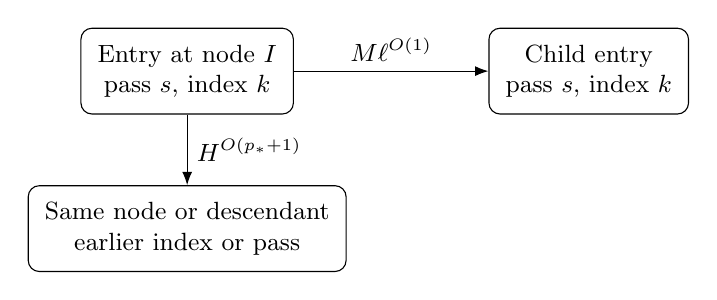
\begin{tikzpicture}[
  box/.style={draw,rounded corners,align=center,inner sep=6pt,font=\small},
  >=Latex]
\node[box] (current) at (0,0) {Entry at node $I$\\pass $s$, index $k$};
\node[box] (child) at (5.1,0) {Child entry\\pass $s$, index $k$};
\node[box] (earlier) at (0,-2) {Same node or descendant\\earlier index or pass};
\draw[->] (current) -- node[above,font=\small] {$M\ell^{O(1)}$} (child);
\draw[->] (current) -- node[right,font=\small] {$H^{O(p_*+1)}$} (earlier);
\end{tikzpicture}
\caption{The two recursive input budgets.  Wide action enumeration and
numerical iterations reuse the gathered inputs and contribute local
work.  Only the horizontal edge keeps both pass and index unchanged.}
\label{fig:dependency-budgets}
\end{figure}

Let $s_{\mathrm{pass}}$ be the number of refinement passes, including
the final pass, and put
\[
 K_{\mathrm{dep}}=s_{\mathrm{pass}}(T+S+1).
\]
A dependency path ending at depth $j$ has at most $j$ same-index
edges, because each descends one level.  It has at most
$K_{\mathrm{dep}}$ other edges: indices strictly decrease between
pass switches, and passes strictly decrease at switches.  Copy
identities do not reset this order.  These bounds hold independently
of every seed or sampling accuracy event.

Unfolding the stored dependency graph only overcounts calculations.
The number of paths ending at depth $j$ is at most
\begin{align}
 &\sum_{r=0}^j\sum_{s=0}^{K_{\mathrm{dep}}}
   \binom{r+s}{r}D_{\mathrm{same}}^r
                       D_{\mathrm{earlier}}^s \notag\\
 &\qquad\le (j+1)(K_{\mathrm{dep}}+1)2^{j+K_{\mathrm{dep}}}
 M^j\ell^{C_1j}H^{C_2(p_*+1)K_{\mathrm{dep}}}.
 \label{eq:dependency-count}
\end{align}
Some index-decreasing edges descend too; ignoring that additional
descent only enlarges this bound.

Write $q_*=p_*+1$.  The parameters and pass count give
\[
 J=O(H/\ell),\qquad
 T=O(H^{3/4})=o(S),\qquad
 K_{\mathrm{dep}}=O\left(\frac{Hq_*}{\ell\log\ell}\right).
\]
Consequently
\begin{align*}
 J\log\ell&=O(H\log\ell/\ell)=o(H),\\
 q_*K_{\mathrm{dep}}\log H
   &=O\left(\frac{Hq_*^2}{\log\ell}\right)=o(H),\\
 J+K_{\mathrm{dep}}&=o(H).
\end{align*}
For the second limit, use
$q_*^2=O(\sqrt{\log\ell}+1)$.  All factors beyond $M^j$ in
\eqref{eq:dependency-count} are therefore $2^{o(H)}$, uniformly for
$0\le j\le J$.  The number of expanded evaluations at depth $j$
is bounded by
\begin{equation}
 M^j2^{o(H)}.
 \label{eq:depth-evaluations}
\end{equation}
This is a deterministic count for the local implementation, not a
count conditioned on the success of its estimates.

\subsection{Expected time and logarithmic-word storage}

\begin{theorem}[Charged expected running time]
\label{thm:work}
The large-input algorithm has worst-case expected running time
$N^{1+o(1)}$ on the logarithmic-word RAM, over its internal
randomness.  This includes input processing, preprocessing, initial
and refined table calculations, all rational arithmetic, sampling,
and data-structure operations.  Its workspace on every execution
is bounded by a fixed polynomial in $N$.  Together with the exact
fallbacks, the same program has the claimed expected asymptotic
bound for each fixed rational $\varepsilon\in(0,1)$.
\end{theorem}

\begin{proof}
Let $n_x=|x|$.  At depth $j$, an interval has width at most
$\ceil{n_x/M^j}$.  Theorem~\ref{thm:seed} bounds the expected cost
of a first initial-entry request there by
\[
 \left(1+\ceil{n_x/M^j}\right)2^{o(H)}.
\]
The conditional first-request argument above makes this valid after
any preceding adaptive execution.  Equivalently, enumerate the
possible request slots in an unfolded computation: at each slot
that requests a new initial entry, condition on the past and use
its independent fresh stream.  The deterministic slot count
\eqref{eq:depth-evaluations} allows the resulting expectations to
be summed.  Repeat requests have only the charged dictionary cost.
The same conditional expectation argument applies to each exact
mixture sampler, whose expected local cost is uniformly bounded.

Combining Lemma~\ref{lem:local-work} with
\eqref{eq:depth-evaluations}, all these costs are at most
\begin{align*}
 2^{o(H)}\sum_{j=0}^J
 M^j\left(1+\ceil{n_x/M^j}\right)
 &\le 2^{o(H)}\sum_{j=0}^J(2M^j+n_x)\\
 &\le 2^{o(H)}\bigl(O(M^J)+(J+1)n_x\bigr)\\
 &\le (n_x+1)2^{o(H)}.
\end{align*}
Here $M^J\le M\max(1,n_x)$ and $M,J=2^{o(H)}$.
No seed or group correctness event was used.  Sorting the occurrence
data and the other input work cost $O(N\log(N+2))$, and leaf queries
cost $O(\log(N+2))$ each.  Since $H=\Theta(\log(N+2))$, the complete
expected bound is $N^{1+o(1)}$.

For storage, the deterministic dependency count bounds the number
of stored table entries by $N^{1+o(1)}$.  Each such evaluation creates
at most $H^{O(p_*+1)}$ auxiliary representative, group and draw
records, so their total satisfies the same bound.  Their keys and
scalar fields have the bit bounds of Lemma~\ref{lem:unconditional-sizes}.
Each local action list and numerical computation has at most
$2^{o(H)}=N^{o(1)}$ scratch size by Lemma~\ref{lem:local-work}; even
retaining such lists or mixtures with their auxiliary records keeps
the total refinement storage at $N^{1+o(1)}$.  A fully expanded initial estimator
also has polynomial worst-case space: its tree has $O(Bn)$ nodes
on padded length $n$, its shift arrays have length $O(n)$, and its
numbers have polynomial bit length in $H$ and $B$.  Pruned arrays
are represented by markers.  Its scratch can be released after
storing the completed integer entry.  Retaining the scratch of
nested calls still gives a polynomial bound, since dependency
depth is at most $J+K_{\mathrm{dep}}$ plus the initial-tree depth.
Rejection loops reuse their buffers and do not enlarge storage
when they run for additional trials.

Thus there is an absolute polynomial space bound in $N$ in the
large branch.  Every workspace address fits a constant number of
$O(\log(N+2))$-bit words.  Larger rational numbers are represented
in multiple such words and processed by charged ordinary integer
algorithms, as used above.  Input symbols and the padding tag also
fit a constant number of these words, with no constant-alphabet
assumption.  The finite parameter-inspection rule and exact
dynamic-programming fallback of Section~\ref{sec:geometry} use
polynomially addressed memory as well.

Finally, for each fixed rational accuracy encoding, its length is
eventually below the inspection limit, and the two remaining
fallback conditions also cease for sufficiently large $N$.
Their sizes are bounded as a function of that fixed parameter.
They do not change the asserted asymptotic bound, although they
impose no efficiency claim uniform in a varying $\varepsilon$.
Together with the success probability established in
Section~\ref{sec:accuracy}, this proves Theorem~\ref{thm:main}.
\end{proof}

\bibliographystyle{plainnat}
\bibliography{references}
\end{document}
